\chapterimage{chap7.jpg}
\chapter{多元函数微分}
\begin{introduction}
	\item 连续、偏导、可微、全微分
	\item 链式法则
	\item 隐函数存在定理
	\item 多元函数极值和最值
	\item 拉格朗日数乘法
\end{introduction}
\section{多元函数微分概念}
\begin{definition}[邻域]
	\begin{enumerate}
		\item $\delta$ 邻域: 设 $P_{0}(x_{0},y_{0})$ 是 $xOy$ 平面上的一个点, $U(P_{0},\delta)$ 表示以 $P_{0}$ 为中心, 
		半径为 $\delta$ 的圆盘, 即 $U(P_{0},\delta) = \{(x,y)|\sqrt{(x-x_{0})^{2}+(y-y_{0})^{2}}<\delta\}$
		\item 去心 $\delta$ 邻域: $\mathring{U}(P_{0},\delta) = \{(x,y)|0<\sqrt{(x-x_{0})^{2}+(y-y_{0})^{2}}<\delta\}$
	\end{enumerate}
\end{definition}
\begin{definition}[多元函数极限]
	设函数 $f(x,y)$ 在区域 $D$ 上有定义, $P_{0}(x_{0},y_{0})\in D$ 或为区域 $D$ 边界上的一点, 如果对于任意给定的正数 $\varepsilon$,
总存 $\delta>0$, 使得当点 $P(x,y)\in D$ 且 $0<\sqrt{(x-x_{0})^{2}+(y-y_{0})^{2}}<\delta$ 时, 对应的函数值 $f(x,y)$ 都满足不等式 
$|f(x,y)-A|<\varepsilon$, 那么称函数 $f(x,y)$ 当 $(x,y)\to(x_{0},y_{0})$ 时的极限为 $A$, 记为 $\lim\limits_{\substack{x\to x_{0}\\y\to y_{0}}}f(x,y)=A$
\end{definition}
\begin{definition}[连续]\label{def: 多元微分学概念: 连续、偏导、可微}
	设函数 $f(x,y)$ 在区域 $D$ 上有定义, $P_{0}(x_{0},y_{0})\in D$ 或为区域 $D$ 边界上的一点, 如果 $\lim\limits_{\substack{x\to x_{0}\\y\to y_{0}}}f(x,y)=f(x_{0},y_{0})$, 
那么称函数 $f(x,y)$ 在点 $(x_{0},y_{0})$ 处连续, 如果函数 $f(x,y)$ 在区域 $D$ 上每一点都连续, 那么称函数 $f(x,y)$ 在区域 $D$ 上连续
\end{definition}
\begin{definition}[偏导数]
	
	设函数 $f(x,y)$ 在 $(x_{0},y_{0})$ 邻域内有定义, 若极限 $\lim\limits_{\Delta x\to 0}\dfrac{f(x_{0}+\Delta x,y_{0})-f(x_{0},y_{0})}{\Delta x}$ 存在,
	我们将这记作 $f(x,y)$ 在 $(x_{0},y_{0})$ 处对 $x$ 的偏导数,记作: 
	$$\dfrac{\partial z}{\partial x}\big|_{\substack{x=x_{0}\\y=y_{0}}}\qquad\qquad 
	\dfrac{\partial f}{\partial x}\big|_{\substack{x=x_{0}\\y=y_{0}}}\qquad\qquad
	z_{x}'\big|_{\substack{x=x_{0}\\y=y_{0}}}$$

	类似地, 可以定义 $f(x,y)$ 在 $(x_{0},y_{0})$ 处对 $y$ 的偏导数, 记作:
	$$\dfrac{\partial z}{\partial y}\big|_{\substack{x=x_{0}\\y=y_{0}}}\qquad\qquad
	\dfrac{\partial f}{\partial y}\big|_{\substack{x=x_{0}\\y=y_{0}}}\qquad\qquad
	z_{y}'\big|_{\substack{x=x_{0}\\y=y_{0}}}$$

	$$f_{x}'(x_{0},y_{0}) = \lim\limits_{\Delta x\to 0}\dfrac{f(x_{0}+\Delta x,y_{0})-f(x_{0},y_{0})}{\Delta x}$$
	$$f_{y}'(x_{0},y_{0}) = \lim\limits_{\Delta y\to 0}\dfrac{f(x_{0},y_{0}+\Delta y)-f(x_{0},y_{0})}{\Delta y}$$
	
	对偏导数进一步求偏导数,可以得到高阶偏导数: $f''_{xx}(x,y),f''_{yy}(x,y),f''_{xy}(x,y),f''_{yx}(x,y)$
\end{definition}
\begin{definition}[可微]
	
	函数 $f(x,y)$ 在点 $(x,y)$ 处的全增量 $\Delta z=f(x+\Delta x,y+\Delta y)-f(x,y)$ 可表示为: 
	$$\Delta z=A\Delta x+B\Delta y+o(\rho)\qquad \rho=\sqrt{(\Delta x)^2+(\Delta y)^2}$$
	
	其中 $A,B$ 只与 $x,y$ 相关, 称 $f(x,y)$ 在点 $(x,y)$ 处可微,$A\Delta x+B\Delta y$ 是 $f(x,y)$ 在点 $(x,y)$ 处的全微分.
	$$dz=A\Delta x+B\Delta y=Adx+Bdy$$
	\begin{enumerate}
		\item 可微必要条件: $f(x,y)$ 在点 $(x,y)$ 处可微 $\Rightarrow$ $f(x,y)$ 在点 $(x,y)$ 处偏导数必定存在且 $\begin{cases} A = \dfrac{\partial z}{\partial x}  \\ B = \dfrac{\partial z}{\partial y}\end{cases}$
		\item 可微充分条件: $f(x,y)$ 在点 $(x,y)$ 处偏导数连续 $\Rightarrow$ $f(x,y)$ 在点 $(x,y)$ 处可微
	\end{enumerate}
\end{definition}
\begin{definition}[偏导数连续性]
	
	$$\begin{cases}
	f'_{x}(x_{0},y_{0}) = \lim\limits_{\Delta x\to 0}\dfrac{f(x_{0}+\Delta x,y_{0})-f(x_{0},y_{0})}{\Delta x} = \lim\limits_{x\to x_{0}} f'_{x}(x,y_{0})\\
	f'_{y}(x_{0},y_{0}) = \lim\limits_{\Delta y\to 0}\dfrac{f(x_{0},y_{0}+\Delta y)-f(x_{0},y_{0})}{\Delta y} = \lim\limits_{y\to y_{0}} f'_{y}(x_{0},y)
	\end{cases}$$
	
	如果这两个极限相等, 就称偏导数在此点连续
\end{definition}
\section{链式法则}

\begin{definition}[链式法则]\label{def: 链式法则}
	$$z=f(u,v),u=\varphi(x,y),v=\phi(x,y)$$
	
	偏导数: 
	$$\dfrac{\partial z}{\partial x}=\dfrac{\partial z}{\partial u}\dfrac{\partial u}{\partial x}+\dfrac{\partial z}{\partial v}\dfrac{\partial v}{\partial x}$$
	$$\dfrac{\partial z}{\partial y}=\dfrac{\partial z}{\partial u}\dfrac{\partial u}{\partial y}+\dfrac{\partial z}{\partial v}\dfrac{\partial v}{\partial y}$$
	
	高阶偏导数: 
	$$\dfrac{\partial^2 z}{\partial x^2}=\left[\dfrac{\partial (\dfrac{\partial z}{\partial u})}{\partial u}\dfrac{\partial u}{\partial x}+\dfrac{\partial (\dfrac{\partial z}{\partial u})}{\partial v}\dfrac{\partial v}{\partial x}\right]\dfrac{\partial u}{\partial x}+
	\dfrac{\partial z}{\partial u}\frac{\partial ^2u}{\partial x^2}+
	\left[\dfrac{\partial (\dfrac{\partial z}{\partial v})}{\partial u}\dfrac{\partial u}{\partial x}+\dfrac{\partial (\dfrac{\partial z}{\partial v})}{\partial v}\dfrac{\partial v}{\partial x}\right]\dfrac{\partial v}{\partial x}+
	\dfrac{\partial z}{\partial v}\frac{\partial ^2v}{\partial x^2}$$
	
	$$\dfrac{\partial^2 z}{\partial y^2}=\left[\dfrac{\partial (\dfrac{\partial z}{\partial u})}{\partial u}\dfrac{\partial u}{\partial y}+\dfrac{\partial (\dfrac{\partial z}{\partial u})}{\partial v}\dfrac{\partial v}{\partial y}\right]\dfrac{\partial u}{\partial y}+
	\dfrac{\partial z}{\partial u}\dfrac{\partial ^2u}{\partial y^2}+
	\left[\dfrac{\partial (\dfrac{\partial z}{\partial v})}{\partial u}\dfrac{\partial u}{\partial y}+\dfrac{\partial (\dfrac{\partial z}{\partial v})}{\partial v}\dfrac{\partial v}{\partial y}\right]\dfrac{\partial v}{\partial y}+
	\dfrac{\partial z}{\partial v}\dfrac{\partial ^2v}{\partial y^2}$$
	
	$$\dfrac{\partial^2 z}{\partial x\partial y}=\left[\dfrac{\partial (\dfrac{\partial z}{\partial u})}{\partial u}\dfrac{\partial u}{\partial y}+\dfrac{\partial (\dfrac{\partial z}{\partial u})}{\partial v}\dfrac{\partial v}{\partial y}\right]\frac{\partial u}{\partial x}+
	\dfrac{\partial z}{\partial u}\dfrac{\partial ^2u}{\partial x\partial y}+
	\left[\dfrac{\partial (\dfrac{\partial z}{\partial v})}{\partial u}\dfrac{\partial u}{\partial y}+\dfrac{\partial (\dfrac{\partial z}{\partial v})}{\partial v}\dfrac{\partial v}{\partial y}\right]\dfrac{\partial v}{\partial x}+
	\dfrac{\partial z}{\partial v}\dfrac{\partial ^2v}{\partial x\partial y}$$

	$$\dfrac{\partial^2 z}{\partial y\partial x}=\left[\dfrac{\partial (\dfrac{\partial z}{\partial u})}{\partial u}\dfrac{\partial u}{\partial x}+\dfrac{\partial (\dfrac{\partial z}{\partial u})}{\partial v}\dfrac{\partial v}{\partial x}\right]\frac{\partial u}{\partial y}+
	\dfrac{\partial z}{\partial u}\dfrac{\partial ^2u}{\partial y\partial x}+
	\left[\dfrac{\partial (\dfrac{\partial z}{\partial v})}{\partial u}\dfrac{\partial u}{\partial x}+\dfrac{\partial (\dfrac{\partial z}{\partial v})}{\partial v}\dfrac{\partial v}{\partial x}\right]\dfrac{\partial v}{\partial y}+
	\dfrac{\partial z}{\partial v}\dfrac{\partial ^2v}{\partial y\partial x}$$

	综上所述, 我们有:
	$$\dfrac{\partial^2 z}{\partial x^2}= \dfrac{\partial ^2z}{\partial u^{2}}(\dfrac{\partial u}{\partial x})^{2}+\dfrac{\partial^{2} z}{\partial u\partial v}\frac{\partial v}{\partial x}\frac{\partial u}{\partial x}+\dfrac{\partial z}{\partial u}\frac{\partial ^2u}{\partial x^2}+
	\dfrac{\partial ^2z}{\partial v\partial u}\dfrac{\partial u}{\partial x}\dfrac{\partial v}{\partial x}+\dfrac{\partial^{2} z}{\partial v^{2}}(\frac{\partial v}{\partial x})^{2}+\dfrac{\partial z}{\partial v}\dfrac{\partial^{2} v}{\partial x^{2}}$$

	$$\dfrac{\partial^2 z}{\partial y^2}= \dfrac{\partial ^2z}{\partial u^{2}}(\dfrac{\partial u}{\partial y})^{2}+\dfrac{\partial^{2} z}{\partial u\partial v}\frac{\partial v}{\partial y}\frac{\partial u}{\partial y}+\dfrac{\partial z}{\partial u}\frac{\partial ^2u}{\partial y^2}+
	\dfrac{\partial ^2z}{\partial v\partial u}\dfrac{\partial u}{\partial y}\dfrac{\partial v}{\partial y}+\dfrac{\partial^{2} z}{\partial v^{2}}(\frac{\partial v}{\partial y})^{2}+\dfrac{\partial z}{\partial v}\dfrac{\partial^{2} v}{\partial y^{2}}$$
	
	$$\dfrac{\partial^2 z}{\partial x\partial y}= \dfrac{\partial ^2z}{\partial u^{2}}\dfrac{\partial u}{\partial y}\dfrac{\partial u}{\partial x}+\dfrac{\partial^{2} z}{\partial u\partial v}\frac{\partial v}{\partial y}\frac{\partial u}{\partial x}+\dfrac{\partial z}{\partial u}\frac{\partial ^2u}{\partial x\partial y}+
	\dfrac{\partial ^2z}{\partial v\partial u}\dfrac{\partial u}{\partial y}\dfrac{\partial v}{\partial x}+\dfrac{\partial^{2} z}{\partial v^{2}}\frac{\partial v}{\partial y}\frac{\partial v}{\partial x}+\dfrac{\partial z}{\partial v}\dfrac{\partial^{2} v}{\partial x\partial y}$$

	$$\dfrac{\partial^2 z}{\partial y\partial x}= \dfrac{\partial ^2z}{\partial u^{2}}\dfrac{\partial u}{\partial x}\dfrac{\partial u}{\partial y}+\dfrac{\partial^{2} z}{\partial u\partial v}\frac{\partial v}{\partial x}\frac{\partial u}{\partial y}+\dfrac{\partial z}{\partial u}\frac{\partial ^2u}{\partial y\partial x}+
	\dfrac{\partial ^2z}{\partial v\partial u}\dfrac{\partial u}{\partial x}\dfrac{\partial v}{\partial y}+\dfrac{\partial^{2} z}{\partial v^{2}}\frac{\partial v}{\partial x}\frac{\partial v}{\partial y}+\dfrac{\partial z}{\partial v}\dfrac{\partial^{2} v}{\partial y\partial x}$$
\end{definition}
\begin{definition}[全微分形式不变性]
	设 $z=f(x,y)$, $x=x(u,v),y=y(u,v)$, 如果 $f(u,v),u(x,y),v(x,y)$ 分别有连续偏导数, 则复合函数 $z=f(u,v)$ 在 $(x,y)$ 处的全微分:
	$$dz=\dfrac{\partial z}{\partial x}dx+\dfrac{\partial z}{\partial y}dy=\dfrac{\partial z}{\partial u}du+\dfrac{\partial z}{\partial v}dv$$
\end{definition}
\section{隐函数存在定理}

\begin{theorem}[隐函数存在定理 1]\label{the: 隐函数存在定理}
	如果函数 $F(x,y)$ 满足一下条件:
	\begin{enumerate}
		\item $F(x_{0},y_{0}) = 0$
		\item $F(x,y)$ 在 $(x_{0},y_{0})$ 的某一个邻域内具有连续偏导数
		\item $F'(x_{0},y_{0})\neq 0$
	\end{enumerate}
	那么方程 $F(x,y)=0$ 在点 $(x_{0},y_{0})$ 的某一个邻域内能够确定唯一的连续且具有连续导数的函数 $y=f(x)$, 满足 $F(x,f(x))=0$ 且 $y_{0} = y(x_{0})$, 且有
	$$\dfrac{dy}{dx} = -\dfrac{F'_{x}}{F'_{y}}$$
\end{theorem}
\begin{theorem}[隐函数存在定理 2]
	如果函数 $F(x,y,z)$ 满足一下条件:
	\begin{enumerate}
		\item $F(x_{0},y_{0},z_{0}) = 0$
		\item $F(x,y,z)$ 在 $(x_{0},y_{0},z_{0})$ 的某一个邻域内具有连续偏导数
		\item $F'(x_{0},y_{0},z_{0})\neq 0$
	\end{enumerate}
	那么方程 $F(x,y,z)=0$ 在点 $(x_{0},y_{0},z_{0})$ 的某一个邻域内能够确定唯一的连续且具有连续导数的函数 $z=f(x,y)$, 满足 $F(x,y,z(x,y))=0$ 且 $z_{0} = z(x_{0},y_{0})$, 且有
	$$\dfrac{\partial z}{\partial x} = -\dfrac{F'_{x}}{F'_{z}}\qquad\qquad \dfrac{\partial z}{\partial y} = -\dfrac{F'_{y}}{F'_{z}}$$
\end{theorem}
\section{多元函数极值和最值}
\begin{definition}[多元函数极值和最值]
	\textbf{极值}

	设函数 $f(x,y)$ 在点 $(x_{0},y_{0})$ 处有定义
	
	1. 如果存在邻域 $U(P_{0},\delta)$, 使得对于任意 $(x,y)\in U(P_{0},\delta)$, 都有 $f(x,y)\leq f(x_{0},y_{0})$, 那么称 $f(x_{0},y_{0})$ 是函数 $f(x,y)$ 的一个极大值
	
	2. 如果存在邻域 $U(P_{0},\delta)$, 使得对于任意 $(x,y)\in U(P_{0},\delta)$, 都有 $f(x,y)\geq f(x_{0},y_{0})$, 那么称 $f(x_{0},y_{0})$ 是函数 $f(x,y)$ 的一个极小值

	\textbf{最值}

	1. 如果对于区域 $D$ 上的任意 $(x,y)$, 都有 $f(x,y)\leq f(x_{0},y_{0})$, 那么称 $f(x_{0},y_{0})$ 是函数 $f(x,y)$ 的一个最大值

	2. 如果对于区域 $D$ 上的任意 $(x,y)$, 都有 $f(x,y)\geq f(x_{0},y_{0})$, 那么称 $f(x_{0},y_{0})$ 是函数 $f(x,y)$ 的一个最小值
\end{definition}
\textbf{无条件极值}
\begin{definition}[多元函数极值]
	二元函数 $f(x,y)$ 在点 $(x_{0},y_{0})$ 取极值的必要条件: 
	$$f'_{x}(x_{0},y_{0})=f'_{y}(x_{0},y_{0})=0$$
	
	二元函数 $f(x,y)$ 在点 $(x_{0},y_{0})$ 取极值的充分条件: 
	$$\begin{cases}
		f_{xx}'(x_{0},y_{0})=A\\
		f_{xy}'(x_{0},y_{0})=B\\
		f_{yy}'(x_{0},y_{0})=C
	\end{cases}  
	\quad \Delta=AC-B^2\Rightarrow
	\begin{cases}
		\Delta>0,\begin{cases} A>0, & \min\\A<0, & \max\end{cases}\\
		\Delta<0, \text{非极值}\\ 
		\Delta=0, \text{方法失效}
	\end{cases}
	$$
\end{definition}
\textbf{条件极值}
\begin{definition}[拉格朗日数乘法]
	
	求目标函数 $u=f(x,y,z)$ 在条件 $\begin{cases}g(x,y,z)=0\\h(x,y,z)=0\end{cases}$ 下的最值
	
	构造辅助函数:  $F(x,y,z,\lambda,\mu)=f(x,y,z)+\lambda g(x,y,z)+\mu h(x,y,z)$
	
	令 $$\begin{cases} F_{x}'=f_{x}'+\lambda g_{x}'+\mu h_{x}'=0\\
		F_{y}'=f_{y}'+\lambda g_{y}'+\mu h_{y}'=0\\
		F_{z}'=f_{z}'+\lambda g_{z}'+\mu h_{z}'=0\\
		F_{\lambda}'= g(x,y,z)=0\\
		F_{\mu}'= h(x,y,z)=0
	\end{cases}$$
	
	得到所有的备选点 $P_{i}$,计算 $f(P_{i})$ 得到最大值和最小值.
\end{definition}
\begin{anymark}[注]
	1. 在不封闭曲线上求最值,可以用拉格朗日数乘法,但是要注意边界条件

	2. 闭区域上多元函数的最值,分为两部分, 第一部分是在区域内部求最值, 第二部分是在区域边界求最值; 前者利用驻点, 后者利用拉格朗日数乘法, 两者结合求最值
\end{anymark}



\chapterimage{chap8.jpg}
\chapter{二重积分}
\begin{introduction}
	\item 二重积分定义
	\item 积分次序
	\item 极坐标和直角坐标下的二重积分
	\item 变量替换
\end{introduction}

\section{二重积分概念和性质}
\begin{definition}[二重积分]
	$f(x,y)$ 是有界闭区域 $D$ 上的有界函数,  将有界闭区域 $D$ 任意分割为 $n$ 个小闭区域
	$$D=\bigcup\limits_{i=1}^{n}D_{i}$$
	$\Delta \sigma_{i}$ 是 $D_{i}$ 的面积, 任取 $(\varepsilon_{i},\eta_{i})\in D_{i}$, 
	作乘积 $f(\varepsilon_{i},\eta_{i})\sigma_{i}$,并求和 $\sum\limits_{i=1}^{n}f(\varepsilon_{i},\eta_{i})\sigma_{i}$, 
	当 $\lim\limits_{n \to +\infty}\{\lambda |\lambda = \max\{d_{i}(i=1,2,\cdots,n)\}, d_{i}\text{是}D_{i}\text{区域的直径}\} = 0$ 时, 极限 $\lim\limits_{\lambda\to 0}\sum\limits_{i=1}^{n}
	f(\varepsilon_{i},\eta_{i})\sigma_{i}$ 存在, 且与 $D$ 的分割方法和 $(\varepsilon_{i},\eta_{i})$ 的取法无关, 那么称此极限
	为 $f(x,y)$ 在区域 $D$ 上的二重积分, 记作 $\iint\limits_{D}f(x,y)d\sigma$

	$$\iint\limits_{D} f(x,y) d\sigma = \lim\limits_{\lambda \to 0}\sum\limits_{i=1}^{n}f(\varepsilon_{i},\eta_{i})\sigma_{i}$$

	其中 $f(x,y)$ 称为被积函数, $f(x,y)ds$ 称为被积表达式, $x,y$ 是积分变量, $D$ 是积分区域

	\textcolor{cyan}{二重积分的几何意义} 
	
	二重积分 $\iint\limits_{D}f(x,y)d\sigma$ 表示区域 $D$ 上以 $f(x,y)$ 为曲顶的曲顶柱体的体积
\end{definition}
\begin{corollary}

	(1). $\iint\limits_{D}1d\sigma = \iint\limits_{D}d\sigma = S_{D}$, $S_{D}$ 是 $D$ 的面积

	(2). $f(x,y)$ 在有界闭区域 $D$ 上可积, $f(x,y)$ 在 $D$ 上必有界

	(3). 积分的线性性质

	$$\iint\limits_{D}\left[k_{1}f(x,y)+k_{2}g(x,y)\right]d\sigma = k_{1}\iint\limits_{D}f(x,y)d\sigma + k_{2}\iint\limits_{D}g(x,y)d\sigma$$

	(4). 积分的可加性

	设 $f(x,y)$ 在有界闭区域 $D$ 内可积, 且 $D_{1}\cup D_{2} = D, D_{1}\cap D_{2} = \emptyset$

	$$\iint\limits_{D}f(x,y)d\sigma = \iint\limits_{D_{1}}f(x,y)d\sigma + \iint\limits_{D_{2}}f(x,y)d\sigma$$

	(5). 积分的保号性
	设 $f(x,y),g(x,y)$ 在有界闭区域 $D$ 内可积, 且 $f(x,y)\leq g(x,y)$

	$$\iint\limits_{D}f(x,y)d\sigma\leq \iint\limits_{D}g(x,y)d\sigma \Rightarrow \big|\iint\limits_{D}f(x,y)d\sigma\big| = \iint\limits_{D}\big|f(x,y)\big|d\sigma$$

	(6). 估值定理

	设 $M,m$ 分别是 $f(x,y)$ 在有界闭区域 $D$ 内的最大值和最小值

	$$mS_{D} \leq \iint\limits_{D}f(x,y)d\sigma \leq M S_{D}$$

	(7). 中值定理

	设 $f(x,y)$ 在有界闭区域 $D$ 内连续

	$$\exists (\xi,\eta)\in D,\ s.t.\ \iint\limits_{D}f(x,y)d\sigma = f(\xi,\eta)S_{D}$$
\end{corollary}

\section{二重积分的对称性}

\begin{theorem}[对称性]
	1. 普通对称性

	(i). 区域 $D$ 关于 $x = a$ 对称, 我们有:
	$$\iint\limits_{D} f(x,y)d\sigma = \begin{cases} 2\iint\limits_{D_{1}} f(x,y)d\sigma & f(2a-x) = f(x) \\ 0 & f(2a-x) = -f(x)  \end{cases}$$
	特别的, 当 $a = 0$ 时, 我们有:
	$$\iint\limits_{D} f(x,y)d\sigma = \begin{cases} 2\iint\limits_{D_{1}} f(x,y)d\sigma & f(-x) = f(x) \\ 0 & f(-x) = -f(x)  \end{cases}$$

	(ii). 区域 $D$ 关于 $y = b$ 对称, 我们有:
	$$\iint\limits_{D} f(x,y)d\sigma = \begin{cases} 2\iint\limits_{D_{1}} f(x,y)d\sigma & f(x,2b-y) = f(x,y) \\ 0 & f(x,2b-y) = -f(x,y)  \end{cases}$$
	特别的, 当 $b = 0$ 时, 我们有:
	$$\iint\limits_{D} f(x,y)d\sigma = \begin{cases} 2\iint\limits_{D_{1}} f(x,y)d\sigma & f(x,-y) = f(x,y) \\ 0 & f(x,-y) = -f(x,y)  \end{cases}$$

	2. 轮换对称性

	区域 $D$ 关于 $x = y$ 对称, 我们有:
	$$\iint\limits_{D} f(x,y)d\sigma = \iint\limits_{D} f(y,x)d\sigma= \dfrac{1}{2}\iint\limits_{D}\left[f(x,y)+f(y,x)\right]d\sigma$$
	$$\iint\limits_{D} f(x,y)d\sigma = \begin{cases} 2\iint\limits_{D_{1}} f(x,y)d\sigma & f(x,y) = f(y,x) \\ 0 & f(x,y) = -f(y,x)  \end{cases}$$

	3. 区域 $D$ 关于原点对称, 我们有:
	$$\iint\limits_{D} f(x,y)d\sigma = \begin{cases} 2\iint\limits_{D_{1}} f(x,y)d\sigma & f(-x,-y) = f(x,y) \\ 0 & f(-x,-y) = -f(x,y)  \end{cases}$$
\end{theorem}
\section{二重积分计算}

\begin{definition}[直角坐标系]
	$$\iint\limits_{D}f(x,y)d\sigma = 
	\begin{cases} 
		\int_{a}^{b}dx\int_{h(x)}^{g(x)}f(x,y)dy \\
		\int_{a}^{b}dy\int_{p(y)}^{q(y)}f(x,y)dx
	\end{cases}$$
\end{definition}

\begin{definition}[极坐标系]
	$$\iint\limits_{D}f(x,y)d\sigma=\iint\limits_{D'}rf(r\cos \theta,r\sin \theta)drd\theta$$
\end{definition}

\begin{definition}[换元法]
	令 $\begin{cases}
	  x = x(u,v)\\
	  y = y(u,v)
	\end{cases}$, 是 $(x,y)$ 面 到 $(u,v)$ 面的一对一映射, 且 $x = x(u,v), y = y(u,v)$ 有一阶连续偏导数
	
	$$J = \big|\dfrac{\partial (x,y)}{\partial (u,v)}\big| = 
	\begin{Vmatrix}
	  \dfrac{\partial x}{\partial u} & \dfrac{\partial x}{\partial v} \\
	  \dfrac{\partial y}{\partial u} & \dfrac{\partial y}{\partial v}
	\end{Vmatrix}
	$$
	$$\iint\limits_{D_{xy}} f(x,y)dxdy = \iint\limits_{D_{uv}} f\left[x(u,v),y(u,v)\right]\cdot Jdudv$$
\end{definition}

\begin{anymark}[变量替换]
	$$d\sigma_{1}=dudv \qquad d\sigma_{2}=|l\times m|$$
	$$\begin{cases}
		x(u,v+dv)-x(u,v)=x'_{v}dv \\
		x(u+du,v)-x(u,v)=x'_{u}du \\
		y(u,v+dv)-y(u,v)=x'_{v}dv \\
		y(u+du,v)-y(u,v)=y'_{u}du
	 \end{cases}\Rightarrow 
	 \begin{cases}
		l=(x'_{u}du,y'_{u}du) \\
		m=(x'_{v}dv,y'_{v}dv)  
	\end{cases}$$
	$$d\sigma_{2}=(x'_{u}y'_{v}-x'_{v}y'_{u})dvdu=\begin{Vmatrix}
			x'_{u} & x'_{v} \\
			y'_{u} & y'_{v}
		\end{Vmatrix}d\sigma_{1}$$
\end{anymark}

\textcolor{cyan}{Example}
\begin{example}[][Exam: 8.3.1]
	$\displaystyle{\int_{0}^{+\infty}e^{-x^{2}}dx}$
\end{example}
\begin{anymark}[证明]
	$I = \int_{0}^{+\infty}e^{-x^{2}}dx = \int_{0}^{+\infty}e^{-y^{2}}dy$

	\begin{eqnarray*}
		I^{2} & = & \int_{0}^{+\infty}e^{-x^{2}}dx\int_{0}^{+\infty}e^{-y^{2}}dy\\
			  & = & \int_{0}^{+\infty}dx\int_{0}^{+\infty}e^{-(x^{2}+y^{2})}dy\\
			  & = & \int_{0}^{\frac{\pi}{2}}d \theta \int_{0}^{+\infty}re^{-r^{2}}dr\\
			  & = & \dfrac{\pi}{4} \\
		I	  & = & \dfrac{\sqrt{\pi}}{2}
	\end{eqnarray*}
\end{anymark}


\begin{example}[][Exam: 8.3.2]
	$\displaystyle{\int_{0}^{a}f(x)dx\int_{0}^{a}\frac{1}{f(x)}dx\geq a^{2}}$
\end{example} 
\begin{anymark}[证明]
	$$I = \int_{0}^{a}f(x)dx\int_{0}^{a}\dfrac{1}{f(x)}dx = \iint\limits_{\substack{0\leq x\leq a\\0\leq y\leq a}}\dfrac{f(x)}{f(y)}dxdy$$

	\begin{eqnarray*}
		2I    & = & \iint\limits_{\substack{0\leq x\leq a\\0\leq y\leq a}}\dfrac{f(x)}{f(y)}dxdy 
				+   \iint\limits_{\substack{0\leq x\leq a\\0\leq y\leq a}}\dfrac{f(y)}{f(x)}dxdy\\
			  & \geq & \iint\limits_{\substack{0\leq x\leq a\\0\leq y\leq a}} 2dxdy\\
			  &  =   & 2a^{2}\\
		 I	  & \geq a^{2}& 
	\end{eqnarray*}
\end{anymark}

\chapterimage{chap9.jpg}
\chapter{常微分方程}
\begin{introduction}
	\item 微分方程概念、解和通解
	\item 一阶微分方程
	\item 伯努利方程
	\item (非)齐次二阶常系数线性微分方程
	\item 欧拉方程
	\item 高阶线性微分方程
\end{introduction}
\begin{definition}[微分方程及其阶]
	表示未知函数及其导数(或者微分)与自变量之间关系的方程称为微分方程, 一般写为:
	$$F(x,y,y',y'',\dots,y^{(n)})=0\text{或} y^{(n)} = f(x,y,y',\cdots,y^{(n-1)})$$
	
	微分方程中未知函数的最高阶导数的阶数称为\textbf{微分方程的阶}.
\end{definition}

\begin{definition}[常微分方程]
	未知函数是一元函数的微分方程称为\textbf{常微分方程}.
\end{definition}

\begin{definition}[线性微分方程]
	$$a_{n}(x)y^{(n)} + a_{n-1}(x)y^{(n-1)} + \cdots + a_{1}(x)y' + a_{0}(x) y = f(x)$$
	形如上述的微分方程称为 $n$ 阶\textbf{线性微分方程}, 其中 $a_{k}(x)(k=0,1,2,\cdots,n)$ 都是自变量 $x$ 的函数, $a_{k}(x)\not\equiv 0$, 当 $a_{k}(x)(k=0,1,2,\cdots,n)$ 都是常数时,
	又称方程为 $n$ 阶\textbf{常系数线性微分方程}; 若右端 $f(x)\equiv 0$, 则称方程为 $n$ 阶\textbf{齐次线性微分方程}, 否则称其为 $n$ 阶\textbf{非齐次线性微分方程}.
\end{definition}
\begin{definition}[微分方程的解和通解]
	\begin{itemize}
		\item 若将函数代入微分方程, 使方程成为恒等式, 则该函数称为\textbf{微分方程的解}, 微分方程解的图形称为积分曲线
		\item 若微分方程的解中含有的独立常数的个数等于微分方程的阶数, 则该解称为微分方程的\textbf{通解}.
	\end{itemize}
\end{definition}
\begin{definition}[初始条件和特解]
	确定通解中常数的条件就是\textbf{初始条件},如 $y(x_{0})=a_{0},y'(x_{0})=a_{1},\cdots,y^{(n-1)}(x_{0})=a_{n-1}$,
	其中 $a_{0},a_{1},\cdots,a_{n-1}$ 为 $n$ 个给定的数, 确定通解中的常数后, 解就成为\textbf{特解}.
\end{definition}
\section{一阶微分方程}

\subsection{可分离变量型微分方程}\label{def: 分离变量型一阶微分方程}
\subsubsection{直接可分离}
$$\dfrac{dy}{dx} = F(x,y)=f(x)g(y)\Rightarrow \int \dfrac{dy}{g(y)} = \int f(x)dx$$
\subsubsection{换元后可分离}

$$\dfrac{dy}{dx} = f(ax+by+c)\Rightarrow 
\begin{cases}
	u = ax +by +c\\
	\dfrac{du}{dx} = a + b\dfrac{dy}{dx}\\
	\dfrac{du}{dx} = a + bf(u)
\end{cases}\Rightarrow \int \dfrac{du}{a + bf(u)} = \int dx$$
\begin{anymark}[注]
	\begin{itemize}
		\item 在换元过程中, 可能会因为定义域问题漏掉某些解, 这些解称为奇解.
		\item 非线性微分方程的所有解等于通解和奇解的并集; 线性微分方程的所有解等于通解, 没有奇解.
	\end{itemize}
\end{anymark}

\subsection{齐次型微分方程}
$$\dfrac{dy}{dx} = \varphi(\dfrac{y}{x})\Rightarrow 
\begin{cases}
	u = \dfrac{y}{x}\\
	\dfrac{dy}{dx} = \dfrac{d(ux)}{x} = u + x\dfrac{du}{dx}\\
	u + x\dfrac{du}{dx} = \varphi(u)
\end{cases}\Rightarrow \int \dfrac{du}{\varphi(u) - u} =\int \dfrac{dx}{x} $$

\subsection{一阶线性微分方程}\label{def: 一阶线性微分方程公式}
\begin{definition}[一阶线性微分方程]
	$$y'+p(x)y=q(x), p(x)\text{和} q(x)\text{是已知的连续函数}$$
\end{definition}
\begin{theorem}[一阶线性微分方程解]
	$$y=e^{-\int p(x)dx}\left[\int e^{\int p(x)dx}q(x)dx+C\right]$$
	\begin{anymark}[注]
		\begin{eqnarray*}
			&\quad & e^{\int p(x)dx}y' + p(x)e^{\int p(x)dx} = q(x)\cdot e^{\int p(x)dx}\\
			&\quad & \left[e^{\int p(x)dx}y\right]' = q(x)\cdot e^{\int p(x)dx}\\
			&\quad & e^{\int p(x)dx}y = \int q(x)\cdot e^{\int p(x)dx} + C\\
			&\quad & y = e^{-\int p(x)dx}\left[\int q(x)\cdot e^{\int p(x)dx} + C\right]
		\end{eqnarray*}
	\end{anymark}
\end{theorem}

\subsection{伯努利方程}
\begin{definition}[伯努利方程]\label{def: 伯努利方程}
	$$\dfrac{dy}{dx}+p(x)y=q(x)y^{n}$$
\end{definition}
\begin{theorem}
	$$y^{-n}\dfrac{dy}{dx} +p(x)y^{1-n} = q(x)\Rightarrow
	\begin{cases}
		z = y^{1-n}\\
		\dfrac{dz}{dx} = \dfrac{1}{1-n}y^{-n}\dfrac{dy}{dx}
	\end{cases}\Rightarrow (1-n)\dfrac{dz}{dx} + p(x)z =q(x)$$

	我们可以得到: 
	$$\dfrac{dz}{dx} + (1-n)p(x)z = (1-n)q(x)\Rightarrow z = e^{-\int (1-n)p(x)dx}\left[ e^{\int (1-n)p(x)dx}\cdot q(x)+ C \right]$$
\end{theorem}

\subsection{二阶可降阶微分方程}
\begin{definition}[二阶可降阶微分方程]

	1. $y''=f(y,y')\Leftrightarrow F(y,y',y'') = 0$

	我们令:  $p=y'$,则 
	$$y''=\frac{dp}{dx}=\frac{dp}{dy}\frac{dy}{dx}=p'p \Rightarrow p\dfrac{dp}{dy} = f(y,p)$$

	2. $y''=f(x,y')\Leftrightarrow F(x,y',y'') = 0$

	我们令:  $p(x)=y'$,则
	$$y''=\frac{dp}{dx}\Rightarrow \dfrac{dp}{dx} = f(x,p)$$
\end{definition}
\section{高阶线性微分方程}
\subsection{二阶常系数线性微分方程}
\begin{definition}[二阶常系数线性微分方程]
	二阶常系数齐次微分方程:
	$$y''+py'+py=0$$
	二阶常系数非齐次微分方程:
	$$y''+py'+py=f(x)$$
\end{definition}
\begin{theorem}[二阶常系数齐次线性微分方程解]\label{the: 齐次二阶常系数线性微分方程}
	对于二阶常系数齐次x线性微分方程:

	特征方程:  $\lambda^{2}+p\lambda+q=0$

	\begin{itemize}
		\item 当方程有两个不同的实数根 $\lambda_{1},\lambda_{2}$ ,微分方程通解: $$y=C_{1}e^{\lambda_{1} x}+C_{2}e^{\lambda_{2}x}$$
		\item 当方程有两个相同的实根 $\lambda_{1}=\lambda_{2}=\lambda$ ,微分方程通解: $$y=C_{1}+C_{2}xe^{\lambda x}$$
		\item 当方程有两个不同的虚根 $\lambda_{1}=\alpha +i\beta,\lambda_{2}=\alpha-i\beta$ ,微分方程通解: $$y=e^{\alpha x}(C_{1}\cos \beta x+C_{2}\sin \beta x)$$
	\end{itemize}
\end{theorem}
\begin{theorem}[二阶常系数非齐次线性微分方程解]
	对于二阶常系数非齐次线性微分方程:
	$$y''+py'+py=f(x)$$
	\textbf{通解为二阶常系数齐次线性微分方程的通解加上特解}: $y_{0}=y^{*}+y$

	1. 当 $f(x)=e^{\alpha x}P_{n}(x)$时,特解 $y^{*}$:

	$$y^{*}=e^{\alpha x}x^{k}Q_{n}(x)$$
	\begin{itemize}
		\item 当 $\alpha$ 不是特征方程的根,$k=0$
		\item 当 $\alpha$ 是特征方程的一个根,$k=1$
		\item 当 $\alpha$ 是特征方程的重根,$k=2$
	\end{itemize}

	2. 当 $f(x)=e^{\alpha x}(P_{n}(x)\cos \beta x+P_{m}(x)\sin \beta x)$时,特解 $y^{*}$:

	$$y^{*}=e^{\alpha x}x^{k}(Q_{l}^{(1)}(x)\cos \beta x+Q_{l}^{(2)}(x)\sin \beta x),\quad l=max\{m,n\}$$
	\begin{itemize}
		\item 当 $\alpha\pm i\beta$ 不是特征方程的根,$k=0$
		\item 当 $\alpha\pm i\beta$ 是特征方程的根,$k=1$
	\end{itemize}
\end{theorem}

\subsection{欧拉方程}
\begin{definition}[欧拉方程]\label{def: 欧拉方程}
	形如以下形式的微分方程:
	$$x^{2}\dfrac{d^{2}y}{dx^2}+px\dfrac{dy}{dx}+qy=f(x)$$

	1. 当 $x>0$ 时,令 $x=e^t,t=\ln x;\dfrac{dt}{dx}=\dfrac{1}{x}$

	$$\dfrac{dy}{dx}=\dfrac{dy}{dt}\dfrac{dt}{dx}=\dfrac{1}{x}\dfrac{dy}{dt}$$
	$$\dfrac{d^{2}y}{dx^2}=\dfrac{d(\frac{dy}{dx})}{dt}\dfrac{dt}{dx}=\dfrac{1}{x^2}\dfrac{d^{2}y}{dt^2}$$

	原微分方程可化为:
	$$\dfrac{d^{2}y}{dt^2}+p\dfrac{dy}{dt}+qy=f(e^t)$$

	2. 当 $x<0$ 时,令 $x=-e^t,t=\ln(-x);\dfrac{dt}{dx}=\dfrac{1}{x}$

	$$\dfrac{dy}{dx}=\dfrac{dy}{dt}\dfrac{dt}{dx}=\dfrac{1}{x}\dfrac{dy}{dt}$$
	$$\dfrac{d^{2}y}{dx^2}=\dfrac{d(\frac{dy}{dx})}{dt}\dfrac{dt}{dx}=\dfrac{1}{x^2}\dfrac{d^{2}y}{dt^2}$$

	原微分方程可化为:
	$$\dfrac{d^{2}y}{dt^2}+p\dfrac{dy}{dt}+qy=f(-e^t)$$
\end{definition}
\subsection{高阶常系数齐次线性微分方程}
\begin{definition}[高阶常系数齐次线性微分方程]
	$n(n\geq 3)$ 阶常系数齐次线性微分方程称为高阶常系数齐次线性微分方程。
\end{definition}

\begin{proposition}[$n$ 阶常系数线性微分方程解]
	特征方程:
	$$a_{0} + a_{1}x + \cdots + a_{n-1}x^{n-1} + a_{n}x^{n} = 0$$

	\begin{enumerate}
		\item $r$ 是单实数根, 通解包含 $Ce^{rx}$
		\item $r$ 是 $k$ 重实数根, 通解包含 $(C_{1} + C_{2}x + C_{3}x^{2} + \cdots + C_{k}x^{k-1})e^{rx}$
		\item $r$ 是单复根, 通解包括 $e^{rx}(C_{1}\cos \beta x+C_{2}\sin \beta x)$
		\item $r$ 是二重复根, 通解包括 $e^{rx}(C_{1}\cos \beta x+C_{2}\sin \beta x+C_{3}x\cos \beta x+C_{4}x\sin \beta x)$
	\end{enumerate}
\end{proposition}

\chapterimage{chap10.jpg}	
\chapter{无穷级数(非数二)}
\begin{introduction}
	\item 常数项级数
	\item 敛散性判别
	\item 收敛域和收敛半径
	\item 函数项级数
	\item 幂级数
	\item 和函数和函数展开式
	\item 傅里叶级数
\end{introduction}
\section{常数项级数}

\begin{definition}[级数定义]
	给定一个无穷数列 $u_{1},u_{2},u_{3},\dots,u_{n},\dots$,将其各项相加得到 $\sum\limits_{n=1}^{+\infty}u_{n}$
	$$u_{1}+u_{2}+u_{3}+\dots+u_{n}+\dots=\sum_{n=1}^{+\infty}u_{n}$$
	我们将 $\sum\limits_{n=1}^{+\infty}u_{n}$ 称为无穷级数,简称为级数,其中 $u_{n}$ 是无穷级数的通项,如果 $u_{n}$ 是常数项,则称为常数项级数;如果 $u_{n}$ 是函数,则称为函数项级数
\end{definition}
\begin{definition}[级数敛散性]
	级数 $\sum\limits_{n=1}^{+\infty}u_{n}$ 的敛散性研究:
	\myspace{1}
	引入 $S_{n}=\sum\limits_{i=1}^{n}u_{i}$,我们称 $S_{n}$ 是无穷级数的部分和,我们定义:
	\myspace{1}
	(1). 当 $\lim\limits_{n\to +\infty}S_{n}=S$ 时,我们称级数 $\sum\limits_{n=1}^{+\infty}u_{n}$ 收敛.
	\myspace{1}
	(2). 当 $\lim\limits_{n\to +\infty}S_{n}=\infty$ 或者不存在时,我们称级数 $\sum\limits_{n=1}^{+\infty}u_{n}$ 发散.
\end{definition}

\begin{corollary}
	(1). 当 $\sum\limits_{n=1}^{+\infty}u_{n}$ 收敛时,我们有:  $\lim\limits_{n\to +\infty}u_{n}=0$ (必要条件)
	\myspace{1}
	(2). 当 $\sum\limits_{n=1}^{+\infty}u_{n},\sum\limits_{n=1}^{+\infty}v_{n}$ 收敛时,且这两个级数的和分别为 $S,T$, $\forall \alpha ,\beta \in \mathbb{R} ,\sum\limits_{n=1}^{+\infty}(\alpha u_{n}+\beta v_{n})$ 收敛,且级数和为 $\alpha S+\beta T$
	\myspace{1}
	(3). 改变级数任意有限项, 不会改变该级数的敛散性
	\myspace{1}
	(4). 收敛级数的任意项加括号所得到的新级数仍收敛, 且其和不变
\end{corollary}

\section{敛散性判别}
\subsection{正项级数判别}\label{the: 正向级数敛散性的判别方法}

(1). 定义法
\begin{theorem}[收敛原则]
	$\sum\limits_{n=1}^{+\infty}u_{n}$ 收敛 $\Leftrightarrow S_{n}$ 有界
\end{theorem}

\begin{proof}
	$\sum\limits_{n=1}^{+\infty}u_{n}$ 是正项级数,$u_{n}\geq 0, S_{n}$ 单调递增

	$S_{n}$ 有界, 单调有界准则: $\lim\limits_{n\to+\infty}S_{n}$ 存在, 原级数收敛
\end{proof}
\myspace{1}

(2). 比较判别法

\begin{theorem}[比较判别法]
	两个正项级数 $\sum\limits_{n=1}^{+\infty}u_{n}$ 和 $\sum\limits_{n=1}^{+\infty}v_{n}$, 若从某一项起满足 $u_{n} \leq v_{n}$:
	\myspace{1}
	若 $\sum\limits_{n=1}^{+\infty}u_{n}$ 发散, $\sum\limits_{n=1}^{+\infty}v_{n}$ 发散
	\myspace{1}
	若 $\sum\limits_{n=1}^{+\infty}v_{n}$ 收敛, $\sum\limits_{n=1}^{+\infty}u_{n}$ 收敛
\end{theorem}

(3). 比较判别法的极限形式

\begin{theorem}[比较判别法的极限形式]\label{the: 比较判别法的极限形式}
	两个正项级数 $\sum\limits_{n=1}^{+\infty}u_{n}$ 和 $\sum\limits_{n=1}^{+\infty}v_{n}(v_{n}\neq 0)$, 且 $\lim\limits_{n\to+\infty}\dfrac{u_{n}}{v_{n}}=A$
	\myspace{1}
	(i). $A=0$,若 $\sum\limits_{n=1}^{+\infty}v_{n}$ 收敛,$\sum\limits_{n=1}^{+\infty}u_{n}$ 收敛

	(ii). $0<A<+\infty$,$\sum\limits_{n=1}^{+\infty}u_{n}$ 和 $\sum\limits_{n=1}^{+\infty}v_{n}$ 有相同的敛散性

	(iii). $A=+\infty$,若 $\sum\limits_{n=1}^{+\infty}v_{n}$ 发散,$\sum\limits_{n=1}^{+\infty}u_{n}$ 发散
\end{theorem}

(4). 比值判别法(达朗贝尔判别法)

\begin{theorem}[比值判别法]
	正项级数 $\sum\limits_{n=1}^{+\infty}u_{n}$, 且 $\lim\limits_{n\to+\infty}\dfrac{u_{n+1}}{u_{n}}=\rho$
	\myspace{1}
	(i). $\rho<1$, $\sum\limits_{n=1}^{+\infty}u_{n}$ 收敛

	(ii). $\rho>1$, $\sum\limits_{n=1}^{+\infty}u_{n}$ 发散

	(iii). $\rho=1$, $\sum\limits_{n=1}^{+\infty}u_{n}$ 敛散性不确定
\end{theorem}

(5). 根值判别法(柯西判别法)

\begin{theorem}[根值判别法]
	正项级数 $\sum\limits_{n=1}^{+\infty}u_{n}$, 且$\lim\limits_{n\to+\infty}\sqrt[n]{u_{n}}=\rho$
	\myspace{1}
	(i). $\rho<1$, $\sum\limits_{n=1}^{+\infty}u_{n}$ 收敛

	(ii). $\rho>1$, $\sum\limits_{n=1}^{+\infty}u_{n}$ 发散

	(iii). $\rho=1$, $\sum\limits_{n=1}^{+\infty}u_{n}$ 敛散性不确定
\end{theorem}

(6). 积分判别法

\begin{theorem}[积分判别法]
	正项级数 $\sum\limits_{n=1}^{+\infty}u_{n}$, 若存在在 $[1,+\infty)$ 上单调减少的非负函数 $f(x)$, 
	使得 $u_{n} = f(n)$, 则级数 $\sum\limits_{n=1}^{+\infty}u_{n}$ 与反常积分 $\int_{1}^{+\infty}f(x)dx$ 敛散性相同

\end{theorem}
\subsection{交错级数判别}

\begin{theorem}[莱布尼茨判别法]
	$u_{n}$ 单调不增且 $\lim\limits_{n\to +\infty}u_{n}=0$  $\Rightarrow\sum\limits_{n=1}^{+\infty}(-1)^{n-1}u_{n}$ 收敛
\end{theorem}

\subsection{一般项级数判别}
\begin{definition}
	$\sum\limits_{n=1}^{+\infty}|u_{n}|$ 是原级数的绝对值级数
	\myspace{1}
	(i). 如果 $\sum\limits_{n=1}^{+\infty}|u_{n}|$ 收敛,称其\textbf{绝对收敛}
	\myspace{1}
	(ii). 如果 $\sum\limits_{n=1}^{+\infty}|u_{n}|$ 发散,$\sum\limits_{n=1}^{+\infty}u_{n}$ 收敛,称其\textbf{条件收敛}
\end{definition}
\subsection{常见级数敛散性推论}
\begin{corollary}
	设 $\sum\limits_{n=1}^{+\infty} u_{n}, \sum\limits_{n=1}^{+\infty}v_{n}, \sum\limits_{n=1}^{+\infty}w_{n}$ 是任意项级数

	$$\begin{cases}
  		v_{n} = \dfrac{u_{n} + |u_{n}|}{2} \\
  		w_{n} = \dfrac{|u_{n}| - u_{n}}{2}
	\end{cases}$$

	(1). $a, b, c$ 是非零常数, 且 $au_{n} + bv_{n} + cw_{n} = 0$, 在 $\sum\limits_{n=1}^{+\infty} u_{n}, \sum\limits_{n=1}^{+\infty}v_{n}, \sum\limits_{n=1}^{+\infty}w_{n}$ 
	中只要有两个级数收敛, 另一个级数必收敛

	(2). 级数 $\sum\limits_{n=1}^{+\infty}|u_{n}|$ 收敛 $\Rightarrow$ 级数 $\sum\limits_{n=1}^{+\infty}u_{n}$ 收敛; 级数 $\sum\limits_{n=1}^{+\infty}u_{n}$ 发散 $\Rightarrow$ 级数 $\sum\limits_{n=1}^{+\infty}|u_{n}|$ 发散

	(3). 级数 $\sum\limits_{n=1}^{+\infty}u^{2}_{n}$ 收敛 $\Rightarrow$ 级数 $\sum\limits_{n=1}^{+\infty}\dfrac{u_{n}}{n}$ 绝对收敛 $\qquad \big|\dfrac{u_{n}}{n}\big| \leq \dfrac{1}{2}(u^{2}+\dfrac{1}{n^{2}})$

	(4).  级数 $\sum\limits_{n=1}^{+\infty}u_{n}$ 收敛, 级数 $\sum\limits_{n=1}^{+\infty}|u_{n}|$ 和级数 $\sum\limits_{n=1}^{+\infty}u^{2}_{n}$ 收敛性不确定 $\qquad u_{n} = (-1)^{n-1}\dfrac{1}{n}$

	(5). 级数 $\sum\limits_{n=1}^{+\infty}u_{n}$ 收敛, 级数 $\sum\limits_{n=1}^{+\infty}(-1)^{n}u_{n}$ 收敛性不确定 $\qquad u_{n} = (-1)^{n}\dfrac{1}{n}$

	(6). 级数 $\sum\limits_{n=1}^{+\infty}u_{n}$ 收敛, 级数 $\sum\limits_{n=1}^{+\infty}(-1)^{n}\dfrac{u_{n}}{n}$ 收敛性不确定 $\qquad u_{n} = (-1)^{n}\dfrac{1}{\ln n}$

	(7). 级数 $\sum\limits_{n=1}^{+\infty}u_{n}$ 收敛, 级数 $\sum\limits_{n=1}^{+\infty}(u_{2n-1}+u_{2n})$ 收敛; 级数 $\sum\limits_{n=1}^{+\infty}u_{2n}$ 和级数 $\sum\limits_{n=1}^{+\infty}u_{2n-1}$ 收敛性不确定
\end{corollary}
\myspace{1}
\section{函数项级数}
\begin{definition}[函数项级数]
	设函数列 $\{u_{n}(x)\}$ 定义在区间 $I$ 上, 称 
	
	$$\sum\limits_{n=1}^{+\infty}u_{n}(x)=u_{1}(x)+u_{2}(x)+u_{3}(x)+\dots+u_{n}(x)+\dots$$
	
	为定义在区间 $I$ 上的 \textbf{函数项级数}, 记作 $\sum\limits_{n=1}^{+\infty}u_{n}(x)$, 当 $x$ 取确定的值 $x_{0}$ 时, 
	$\sum\limits_{n=1}^{+\infty}u_{n}(x)$ 成为常数项级数 $\sum\limits_{n=1}^{+\infty}u_{n}(x_{0})$
\end{definition}
\begin{definition}[收敛点和发散点]
	(1). 若给定 $x_{0}\in I$, 有 $\sum\limits_{n=1}^{+\infty}u_{n}(x_{0})$ 收敛, 
	则称 $x=x_{0}$ 是函数项级数 $\sum\limits_{n=1}^{+\infty}u_{n}(x)$ 的\textbf{收敛点}

	(2). 若 $\sum\limits_{n=1}^{+\infty}u_{n}(x_{0})$ 发散, 则称  $x = x_{0}$ 是函数项级数 $\sum\limits_{n=1}^{+\infty}u_{n}(x)$ 的\textbf{发散点}
\end{definition}

\begin{definition}[收敛域]
	函数项级数 $\sum\limits_{n=1}^{+\infty}u_{n}(x)$ 的所有收敛点的集合称为函数项级数 $\sum\limits_{n=1}^{+\infty}u_{n}(x)$ 的 \textbf{收敛域}
\end{definition}
\subsection{幂级数}

\begin{definition}[幂级数]
	若 $\sum\limits_{n=0}^{+\infty}u_{n}(x)$ 的一般项 $u_{n}(x)$ 是 $x$ 的 $n$ 次幂函数, 
	则称 $\sum\limits_{n=0}^{+\infty}u_{n}(x)$ 为\textbf{幂级数}
	\myspace{1}
	标准形式:
	$$\sum\limits_{n=0}^{+\infty}u_{n}(x)=a_{0}+a_{1}x+a_{2}x^{2}+\dots+a_{n}x^{n}+\dots$$
	
	一般形式:
	$$\sum\limits_{n=0}^{+\infty}u_{n}(x)=a_{0}+a_{1}(x-x_{0})+a_{2}(x-x_{0})^{2}+\dots+a_{n}(x-x_{0})^{n}+\dots$$

	其中 $a_{n}(n=0,1,2\cdots)$ 为\textbf{幂级数的系数}  
\end{definition}

\subsection{幂级数收敛域}
\begin{theorem}[阿贝尔定理]
	\textbf{阿贝尔定理}
	\myspace{1}
	当幂级数 $\sum\limits_{n=0}^{+\infty}a_{n}x^{n}$ 在 $x=x_{1}(x_{1}\neq 0)$ 处收敛时, $\forall x < |x_{1}|$, 幂级数 $\sum\limits_{n=0}^{+\infty}a_{n}x^{n}$ 都收敛

	当幂级数 $\sum\limits_{n=0}^{+\infty}a_{n}x^{n}$ 在 $x=x_{2}(x_{2}\neq 0)$ 处发散时, $\forall x > |x_{2}|$, 幂级数 $\sum\limits_{n=0}^{+\infty}a_{n}x^{n}$ 都发散
\end{theorem}

\begin{theorem}[收敛域和收敛半径]
	(1). 不缺项幂级数(\textbf{充分条件}): 
	$$\lim\limits_{n\to +\infty}|\dfrac{a_{n+1}}{a_{n}}|=\rho$$
	
	$$R = \begin{cases}
		\dfrac{1}{\rho},\rho \neq 0 \\
		0,\rho = \infty            \\
		\infty,\rho = 0
	\end{cases}$$

	区间 $(-R,R)$ 是幂级数 $\sum\limits_{n=0}^{+\infty}a_{n}x^{n}$ 的收敛区间; 
	幂级数的收敛域为 $(-R,R) \ or \ [-R,R]\ or\ (-R,R] \ or\ [-R,R) $

	(2). 缺项幂级数或一般项级数 $\sum\limits_{n=1}^{+\infty}u_{n}(x)$, 利用正项级数判别法中的比值判别法(\textbf{充分条件}):
	$$\rho(x) = \begin{cases}
		\lim\limits_{n \to +\infty} \big|\dfrac{u_{n+1}(x)}{u_{n}(x)}\big| < 1\\
		\lim\limits_{n \to +\infty}\sqrt[n]{u_{n}(x)} < 1
	\end{cases}\Rightarrow
	x\in (a,b)
	$$
	$$\sum\limits_{n=1}^{+\infty}u_{n}(a)\text{和}\sum\limits_{n=1}^{+\infty}u_{n}(b) \text{敛散性}$$

	(3). 对级数提出或者乘以因式 $(x-x_{0})^{k}$ 或者平移, 收敛半径不变

	(4). 对级数逐项求导, 收敛半径不变, 收敛域可能缩小

	(5). 对级数逐项积分, 收敛半径不变, 收敛域可能扩大
\end{theorem}

\myspace{1}

\subsection{幂级数求和函数}
\begin{definition}[幂级数的和函数]
	在幂级数收敛域上, 记 $S(x)$ 是幂级数的和函数:
	$$S(x)=\sum\limits_{n=0}^{+\infty}u_{n}(x)$$
\end{definition}
\begin{theorem}[运算法则]
	幂级数 $\sum\limits_{n=0}^{+\infty}a_{n}x^{n}$ 与 $\sum\limits_{n=0}^{+\infty}b_{n}x^{n}$ 的收敛半径分别为 $R_{a}$ 和 $R_{b}$, 且 $R_{a}\neq R_{b}$

	(i). $$k \sum\limits_{n=0}^{n}a_{n}x^{n} = \sum\limits_{n=0}^{n}ka_{n}x^{n}, |x| < R_{a}$$

	(ii). $$\sum\limits_{n=0}^{n}a_{n}x^{n} \pm \sum\limits_{n=0}^{n}b_{n}x^{n} = \sum\limits_{n=0}^{n}(a_{n}\pm b_{n})x^{n}, |x| < \min\{R_{a}, R_{b}\}$$

	(iii). $$\sum\limits_{n=0}^{n}a_{n}x^{n}\sum\limits_{n=0}^{n}b_{n}x^{n} = \sum\limits_{n=0}^{n} \left(\sum\limits_{i=0}^{n}a_{i}b_{n-i}\right) x^{n}$$
\end{theorem}

\begin{corollary}
	
	(i). 幂级数 $\sum\limits_{n=0}^{+\infty}a_{n}x^{n}$ 的和函数 $S(x)$ 在其收敛域 $I$ 上连续

	(ii). 幂级数 $\sum\limits_{n=0}^{+\infty}a_{n}x^{n}$ 的和函数 $S(x)$ 在其收敛域 $I$ 上可积分, 且有逐项积分公式, 收敛半径不变, 收敛域可能变大 
	$$\int_{0}^{x}S(t)dt = \int_{0}^{x}\left(\sum\limits_{n=0}^{+\infty}a_{n}t^{n}\right)dt = \sum\limits_{n=0}^{+\infty}a_{n}\int_{0}^{x}t^{n}dt = \sum\limits_{n=0}^{+\infty}\dfrac{a_{n}}{n+1}x^{n+1}(x\in I)$$
	
	(iii). 幂级数 $\sum\limits_{n=0}^{+\infty}a_{n}x^{n}$ 的和函数 $S(x)$ 在其收敛区间 $(-R,R)$ 上可导, 且有逐项求导公式, 收敛半径不变, 收敛域可能变小 
	$$S'(x) = \left(\sum\limits_{n=0}^{+\infty}a_{n}x^{n}\right)' = \sum\limits_{n=0}^{+\infty}\left(a_{n}x^{n}\right)' = \sum\limits_{n=1}^{+\infty}na_{n}x^{n-1}(|x| < R)$$
\end{corollary}

\subsection{重要展开式}

\begin{theorem}\label{the: 重要幂级数展开式}
	$$e^{x}=1+x+\dfrac{x^2}{2!}+\cdots+\dfrac{x^n}{n!}+\cdots = 
	\sum\limits_{n=0}^{+\infty}\dfrac{x^{n}}{n!}, -\infty<x<+\infty$$

	$$\dfrac{1}{1-x}=1+x+x^2+\cdots+x^{n}+\cdots = 
	\sum\limits_{n=0}^{+\infty}x^{n}, -1<x<1$$

	$$\dfrac{1}{1+x}=1-x+x^2-x^3+\cdots+(-1)^{n}x^{n}+\cdots = 
	\sum\limits_{n=0}^{+\infty}(-1)^{n}x^{n},-1<x<1$$

	$$\ln(1+x)=x-\dfrac{x^2}{2}+\dfrac{x^3}{3}-\cdots + \dfrac{(-1)^{n-1}x^{n}}{n}+\cdots
	= \sum\limits_{n=1}^{+\infty}(-1)^{n-1}\dfrac{x^{n}}{n},-1<x\leq 1$$
	
	$$\sin x=x-\dfrac{x^3}{3!}+\dfrac{x^5}{5!}-\cdots+\dfrac{(-1)^{n}x^{2n+1}}{(2n+1)!}+\cdots=\sum\limits_{n=0}^{+\infty}(-1)^{n}\dfrac{x^{2n+1}}{(2n+1)!}, -\infty<x<+\infty$$
	
	$$\cos x=1-\dfrac{x^2}{2!}+\dfrac{x^4}{4!}+\cdots+\dfrac{(-1)^nx^{2n}}{2n!}+\cdots=\sum\limits_{n=0}^{+\infty}(-1)^{n}\dfrac{x^{2n}}{(2n)!}, -\infty<x<+\infty$$
	
	$$\tan x=\sum\limits_{n=0}^{+\infty}(-1)^{n}\dfrac{x^{2n+1}}{2n+1}, -1\leq x\leq 1 $$
	\begin{eqnarray*}
		(1+x)^{\alpha} & = & 1+\alpha x+\dfrac{\alpha (\alpha-1)}{2!}x^2+ \cdots + \dfrac{\alpha (\alpha-1)(\alpha-2)\dots(\alpha-n+1)}{n!}x^n+\cdots\\
		               & = & \begin{cases}
						 x\in (-1,1), & \alpha \leq -1\\
						 x\in (-1,1], & -1 < \alpha < 0\\
						 x\in [-1,1], & \alpha > 0\ \&\ \alpha \notin \mathbb{N}_{+}\\
						 x\in (-\infty,+\infty), & \alpha \in \mathbb{N}_{+}  
					   \end{cases}
	\end{eqnarray*}
\end{theorem}
\subsection{函数展开成幂级数}

\begin{definition}
	\textbf{泰勒级数}: $f(x)$ 在点 $x=x_{0}$ 处存在任意阶导数
	$$f(x)=\sum\limits_{n=0}^{+\infty}\frac{f^{(n)}(x_{0})}{n!}(x-x_{0})^n$$
	\textbf{麦克劳林级数}: $f(x)$ 在点 $x=0$ 处存在任意阶导数
	$$f(x)=\sum\limits_{n=0}^{+\infty}\frac{f^{(n)}(0)}{n!}x^n$$
\end{definition}
\section{傅里叶级数}

\begin{definition}[傅里叶级数]\label{def: 傅里叶级数}
	考虑到三角函数是周期函数, 任意一个以 $2\pi$ 为周期的函数 $f(x)$, 能写成一系列三角函数 $\sin (nx)$ 和 $\cos (nx)$ 的线性组合:

	$$f(x) = \dfrac{a_{0}}{2} + \sum\limits_{n=1}^{+\infty}(a_{n}\cos (nx)+b_{n}\sin (nx))$$

	$f(x)$ 三角函数分解被称为傅里叶级数或傅里叶展开, 也被称为三角级数 
\end{definition}
\subsection{三角函数集 $\Gamma$ 的归一正交性}
\begin{definition}[内积、正交和范数]
	考虑 $[-\pi,\pi]$ 上的函数 $f(x)$ 构成的无限维空间, 我们希望用正交的向量组来表示一般的向量(函数), 我们定义函数内积、正交和范数概念

	(1). 内积
	
	$$\forall f,g \in V, (f\cdot g) = \int_{-\pi}^{\pi}f(x)g(x)dx $$

	(2). 正交

	$$\forall f,g \in V, (f\cdot g) = \int_{-\pi}^{\pi}f(x)g(x)dx = 0\Rightarrow f \bot g $$

	(3). 范数

	$$\forall f \in V, \parallel f \parallel  = \left(\int_{-\pi}^{\pi}f^{2}(x)dx\right)^{\frac{1}{2}}$$
\end{definition}

\begin{definition}[三角函数集 $\Gamma$ 的归一正交性]
	定义在 $[-\pi,\pi]$ 上的函数空间中存在一系列范数为 $1$ 且正交的向量组, 考虑 $[-\pi,\pi]$ 上的三角函数组
	
	$$\Gamma = \left\{\dfrac{1}{\sqrt{2}}, \dfrac{1}{\sqrt{\pi}}\cos x, \dfrac{1}{\sqrt{\pi}}\sin x, \cdots, \dfrac{1}{\sqrt{\pi}}\sin nx, \dfrac{1}{\sqrt{\pi}}\cos nx, \cdots\right\}$$
	
	$$\forall f \in \Gamma, \parallel f \parallel = 1, \forall f,g \in \Gamma, f \cdot g = 0\Rightarrow f \bot g$$

	不妨设 $$\begin{cases}
		f_{1} = \dfrac{1}{\sqrt{\pi}}\sin mx\\
		f_{2} = \dfrac{1}{\sqrt{\pi}}\sin nx
	\end{cases}\qquad 
	\begin{cases}
	  g_{1} = \dfrac{1}{\sqrt{\pi}} \cos mx\\
	  g_{2} = \dfrac{1}{\sqrt{\pi}} \cos nx
	\end{cases}$$

	$$ \begin{cases}
		\parallel f_{1} \parallel = \left(\displaystyle{\int_{-\pi}^{\pi}\sin^{2} nxdx}\right)^{\frac{1}{2}} = 1\\
		\parallel g_{1} \parallel = \left(\displaystyle{\int_{-\pi}^{\pi}\cos^{2} mxdx}\right)^{\frac{1}{2}} = 1
	\end{cases} \qquad
	 \begin{cases}
		f_{1} \cdot g_{1} = \dfrac{1}{\pi}\displaystyle{\int_{-\pi}^{\pi}\sin mx\cos mxdx} = 0 \\
		f_{1} \cdot f_{2} = \dfrac{1}{\pi}\displaystyle{\int_{-\pi}^{\pi}\sin mx\sin nxdx} = 0 (m\neq n)\\
		g_{1} \cdot g_{2} = \dfrac{1}{\pi}\displaystyle{\int_{-\pi}^{\pi}\cos mx\cos nxdx} = 0 (m\neq n)
	 \end{cases}$$
\end{definition}

\subsection{周期函数的傅里叶级数}
\begin{theorem}[周期为 $2\pi$ 函数的傅里叶级数]
	$$f(x) = \dfrac{a_{0}}{2} + \sum\limits_{n=1}^{+\infty}(a_{n}\cos (nx)+b_{n}\sin (nx))$$

	三角函数分解, $a_{n}, b_{n}$ 是傅里叶级数系数:
	$$\begin{cases}
	  \displaystyle{\int_{-\pi}^{\pi}f(x)\cos nx dx = \int_{-\pi}^{\pi}a_{n}\cos^{2} nxdx} \\
	  \displaystyle{\int_{-\pi}^{\pi}f(x)\sin nx dx = \int_{-\pi}^{\pi}b_{n}\sin^{2} nxdx}
	\end{cases}\Rightarrow 
	\begin{cases}
	  \displaystyle{a_{n} = \dfrac{1}{\pi}\int_{-\pi}^{\pi}f(x)\cos nxdx} \\
	  \displaystyle{b_{n} = \dfrac{1}{\pi}\int_{-\pi}^{\pi}f(x)\sin nxdx}
	\end{cases}$$

	记作: \textbf{$2\pi$ 周期函数 $f(x)$ 的傅里叶级数}
	 $$f(x) \sim\dfrac{a_{0}}{2} + \sum\limits_{n=1}^{+\infty}(a_{n}\cos (nx)+b_{n}\sin (nx))$$
\end{theorem}

\begin{theorem}[周期为 $2\pi$ 奇偶函数的傅里叶级数]
	
	(1). $f(x)$ 在 $[-\pi,\pi]$ 为奇函数, 傅里叶级数为\textbf{正弦级数}:
	$$f(x) \sim \sum\limits_{n=1}^{+\infty}b_{n}\sin nx\Rightarrow b_{n} = \dfrac{2}{\pi}\int_{0}^{\pi}f(x)\sin nxdx$$

	(2). $f(x)$ 在 $[-\pi,\pi]$ 为偶函数, 傅里叶级数为\textbf{余弦级数}:
	$$f(x) \sim \dfrac{a_{0}}{2} + \sum\limits_{n=1}^{+\infty}a_{n}\cos nx\Rightarrow a_{n} = \dfrac{2}{\pi}\int_{0}^{\pi}f(x)\cos nxdx$$
\end{theorem}

\subsection{任意对称区间中的傅里叶展开}

\begin{definition}[任意对称区间中的傅里叶展开]
	设 $f(x)$ 定义域为 $[-l,l]$, 令 $y = \dfrac{x\pi}{l},y\in[-\pi,\pi]$

	$$g(y) = \dfrac{a_{0}}{2} + \sum\limits_{n=1}^{+\infty}(a_{n}\cos ny+b_{n}\sin ny)\Rightarrow 
	f(x) = \frac{a_{0}}{2}+\sum\limits_{n=1}^{+\infty}(a_{n}\cos \dfrac{n\pi}{l}x+b_{n}\sin \dfrac{n\pi}{l}x)$$
	
	傅里叶系数:
	
	$$\begin{cases}
		\displaystyle{a_{n}=\dfrac{1}{l}\int_{-l}^{l}f(x)\cos \dfrac{n\pi}{l}xdx}, &n=0,1,2,\cdots \\
		\displaystyle{b_{n}=\dfrac{1}{l}\int_{-l}^{l}f(x)\sin \dfrac{n\pi}{l}xdx}, &n=1,2,\cdots
	\end{cases}$$
\end{definition}

\subsection{周期延拓}
\begin{definition}[周期延拓]
	(1). 周期延拓: $[-\pi,\pi] \to (-\infty,+\infty)$

	(2). 奇延拓: $[0,\pi] \to [-\pi,\pi]$ 且 $f(x)$ 为奇函数, 正弦级数

	(3). 偶延拓: $[0,\pi] \to [-\pi,\pi]$ 且 $f(x)$ 为偶函数, 余弦级数
\end{definition}

\subsection{逐点收敛性理论}
\begin{theorem}[狄利克雷收敛定理]
$f(x)$ 以 $2l$ 为周期的可积函数, 在 $[-l,l]$ 上 $f(x)$ 满足条件:

(1). 连续或者只有有限个第一类间断点

(2). 至多有有限个极值点

$f(x)$ 的傅里叶级数在 $[-l,l]$ 上处处收敛, 其和函数 $S(x)$ 满足 

$$S(x) = \begin{cases}
			f(x),                          & x\text{为连续点}\\
			\dfrac{f(x_{-})+f(x_{+})}{2},  & x \text{为间断点}\\
			\dfrac{f(-l_{+})+f(l_{-})}{2}, & x = \pm l  
		\end{cases}$$
\end{theorem}
\begin{theorem}[帕塞瓦尔公式]
	$f(x)$ 是 $2\pi$ 周期函数, $f(x)$ 在 $[-\pi,\pi]$ 有界可积, 傅里叶系数满足:
	$$\dfrac{a_{0}^{2}}{2} + \sum\limits_{n=1}^{+\infty}(a_{n}^{2}+b_{n}^{2}) = \dfrac{1}{\pi}\int_{-\pi}^{\pi}f^{2}(x)dx$$
\end{theorem}

\begin{corollary}[常见级数和]
(1). $\sum\limits_{n=0}^{+\infty}\dfrac{1}{n!} = e$

(2). $\sum\limits_{n=1}^{+\infty}\dfrac{1}{n^{2}} = \dfrac{\pi^{2}}{6}$

(3). $\sum\limits_{n=1}^{+\infty}\dfrac{1}{n\cdot 2^{n}} = \ln 2$

(4). $\sum\limits_{n=1}^{+\infty}\dfrac{n}{2^{n}} = 2$

(5). $\sum\limits_{n=1}^{+\infty}\dfrac{1}{(2n)!} = \dfrac{e+e^{-1}}{2}$

(6). $\sum\limits_{n=0}^{+\infty}\dfrac{(-1)^{n}}{2n+1} = \dfrac{\pi}{4}$

(7). $\sum\limits_{n=0}^{+\infty}(-1)^{n}\dfrac{2n+2}{(2n+1)!} = \sin 1 + \cos 1$
\end{corollary}

\chapterimage{chap11.jpg}
\chapter{空间解析几何(非数二)}
\section{向量代数}
\begin{definition}[向量代数]
	(1). 方向角: 非零向量 $\boldsymbol{a} = (a_{x},a_{y},a_{z})$ 与 $x,y,z$ 轴所成夹角 $\alpha,\beta,\gamma$ 称为向量 $\boldsymbol{a}$ 的方向角 
	
	(2). 方向余弦: $\cos \alpha,\cos \beta,\cos\gamma$ 称为向量 $\boldsymbol{a}$ 的方向余弦, $\boldsymbol{a} = x\boldsymbol{i} + y\boldsymbol{j} + z\boldsymbol{k}$
	$$\begin{cases}
		\cos \alpha=\dfrac{a_{x}}{|\boldsymbol{a}|} = \dfrac{x}{\sqrt{x^{2}+y^{2}+z^{2}}}\\
		\cos \beta=\dfrac{a_{y}}{|\boldsymbol{a}|} = \dfrac{y}{\sqrt{x^{2}+y^{2}+z^{2}}}\\
		\cos \gamma=\dfrac{a_{z}}{|\boldsymbol{a}|} = \dfrac{z}{\sqrt{x^{2}+y^{2}+z^{2}}}
	\end{cases}$$

	设 $\boldsymbol{a} = (a_{x},a_{y},a_{z}), \boldsymbol{b} = (b_{x},b_{y},b_{z})$

	(3). 夹角
	$$\boldsymbol{a}\cdot \boldsymbol{b} = |\boldsymbol{a}||\boldsymbol{b}|\cos \theta = a_{x}b_{x}+a_{y}b_{y}+a_{z}b_{z}$$
	$$\cos \theta = \dfrac{\boldsymbol{a}\cdot \boldsymbol{b}}{|\boldsymbol{a}||\boldsymbol{b}|} = \dfrac{a_{x}b_{x}+a_{y}b_{y}+a_{z}b_{z}}{\sqrt{a_{x}^2+a_{y}^2+a_{z}^2}\sqrt{b_{x}^2+b_{y}^2+b_{z}^2}}$$
	
	(4). 投影

	$$\textbf{Prj}_{b}\boldsymbol{a}=\dfrac{\boldsymbol{a}\cdot \boldsymbol{b}}{|\boldsymbol{b}|}=\dfrac{a_{x}b_{x}+a_{y}b_{y}+a_{z}b_{z}}{\sqrt{b_{x}^2+b_{y}^2+b_{z}^2}}$$\

	(5). 叉积

	$$\boldsymbol{a}\times \boldsymbol{b} = \begin{vmatrix}
		\boldsymbol{i} & \boldsymbol{j} & \boldsymbol{k} \\
		a_{x} & a_{y} & a_{z} \\
		b_{x} & b_{y} & b_{z}
	\end{vmatrix}$$
	
	$$|\boldsymbol{a}\times \boldsymbol{b}| = |\boldsymbol{a}||\boldsymbol{b}|\sin\theta$$
\end{definition}

\section{空间平面和直线}

\subsection{平面}

\begin{definition}[平面方程]
	
	假设平面的法向量 $\boldsymbol{n} = (A, B. C)$

	(1). 一般式
	
	$$Ax+By+Cz+D=0$$

	
	(2). 点法式
	
	$$A(x-x_{0})+B(y-y_{0}+C(z-z_{0})=0$$
	
	(3). 截距式, 平面过 $(a,0,0), (0,b,0), (0,0,c)$ 三点
	
	$$\dfrac{x}{a}+\dfrac{y}{b}+\dfrac{z}{c}=1$$	
	
	(4). 三点式 $P_{i} (x_{i}, y_{i}, x_{i})(i = 1,2,3)$ 不共线  
	
	$$\begin{vmatrix}
		x-x_{1} & y-y_{1} & z-z_{1}\\
		x-x_{2} & y-y_{2} & z-z_{2}\\
		x-x_{3} & y-y_{3} & z-z_{3}
	\end{vmatrix} = 0$$
\end{definition}

\subsection{直线}

\begin{definition}[直线方程]
	
	假设直线的方向向量 $\boldsymbol{\tau} = (l,m,n)$, $P(x_{0},y_{0},z_{0})$ 是直线上的一点

	(1). 一般式
	
	$$\begin{cases}
		A_{1}x+B_{1}y+C_{1}z + D_{1}= 0, & \boldsymbol{n}_{1}=(A_{1},B_{1},C_{1})\\
		A_{2}x+B_{2}y+C_{2}z + D_{2}= 0, & \boldsymbol{n}_{2}=(A_{2},B_{2},C_{2})\\
		\boldsymbol{\tau} = \boldsymbol{n}_{1}\times \boldsymbol{n}_{2} 
	\end{cases}$$
	
	(2). 点向式
	
	$$\dfrac{x-x_{0}}{l}=\dfrac{y-y_{0}}{m}=\dfrac{z-z_{0}}{n}$$
	
	(3). 参数式
	
	$$\begin{cases}
		x = x_{0} + lt\\
		y = y_{0} + mt\\
		z = z_{0} + nt
	\end{cases}$$
	
	(4). 两点式
	
	$$\dfrac{x-x_{0}}{x_{1}-x_{2}}=\dfrac{y-y_{0}}{y_{1}-y_{2}}=\dfrac{z-z_{0}}{z_{1}-z_{2}}$$
\end{definition}

\begin{theorem}[位置关系]

	(1). 点到直线的距离公式

	点 $M(x, y, z)$ 到直线 $L: \dfrac{x-x_{0}}{l} = \dfrac{y-y_{0}}{m} = \dfrac{z-z_{0}}{n}$ 的距离

	$$d=\dfrac{|\boldsymbol{\tau}\times \overrightarrow{M_{0}M}|}{|\boldsymbol{\tau}|} = \dfrac{\begin{Vmatrix}
		\boldsymbol{i} & \boldsymbol{j} & \boldsymbol{k} \\
		l & m & n \\
		x-x_{0} & y-y_{0} & z-z_{0}
	\end{Vmatrix}}{\sqrt{l^2+m^2+n^2}}$$
	二维平面: $$d = \dfrac{|Ax + By + C |}{\sqrt{A^{2}+B^{2}}}$$
	
	(2). 点到平面距离公式

	点 $P_{0}(x_{0}, y_{0}, z_{0})$ 到平面 $Ax+By+Cz+D=0$ 的距离, $P(x,y,z)$ 是平面上任意一点

	$$d = |\textbf{Prj}_{n}\overrightarrow{P_{0}P}| = \dfrac{|A(x-x_{0})+B(y-y_{0})+C(z-z_{0})|}{\sqrt{A^{2}+B^{2}+C^{2}}} = \dfrac{|Ax+By+Cz+D|}{\sqrt{A^{2}+B^{2}+C^{2}}}{}$$

	(3). 直线和直线

	设 $\boldsymbol{\tau}_{1}(l_{1},m_{1},n_{1}), \boldsymbol{\tau}_{2}(l_{2},m_{2},n_{2})$ 分别是 $L_{1}, L_{2}$ 的方向向量

	$$\begin{cases}
		L_{1} \perp L_{2}\Leftrightarrow \boldsymbol{\tau}_{1} \perp \boldsymbol{\tau}_{2}\Leftrightarrow l_{1}l_{2}+m_{1}m_{2}+n_{1}n_{2}=0\\
		L_{1} \parallel L_{2}\Leftrightarrow \boldsymbol{\tau}_{1} \parallel \boldsymbol{\tau}_{2}\Leftrightarrow \dfrac{l_{1}}{l_{2}} = \dfrac{m_{1}}{m_{2}} = \dfrac{n_{1}}{n_{2}}
	\end{cases}$$

	$L_{1}, L_{2}$ 的夹角 $\theta = \arccos \dfrac{|\boldsymbol{\tau}_{1}\cdot\boldsymbol{\tau}_{2}|}{|\boldsymbol{\tau}_{1}||\boldsymbol{\tau}_{2}|}, \theta \in [0, \dfrac{\pi}{2}]$

	(4). 平面和平面

	设 $\boldsymbol{n}_{1}(A_{1},B_{1},C_{1}), \boldsymbol{n}_{2}(A_{2},B_{2},C_{2})$ 分别是 $\pi_{1}, \pi_{2}$ 的法向量
	
	$$\begin{cases}
		\pi_{1} \perp \pi_{2}\Leftrightarrow \boldsymbol{n}_{1} \perp \boldsymbol{n}_{2}\Leftrightarrow A_{1}A_{2}+B_{1}B_{2}+C_{1}C_{2}=0\\
		\pi_{1} \parallel \pi_{2}\Leftrightarrow \boldsymbol{n}_{1} \parallel \boldsymbol{n}_{2}\Leftrightarrow \dfrac{A_{1}}{A_{2}} = \dfrac{B_{1}}{B_{2}} = \dfrac{C_{1}}{C_{2}}\\
	\end{cases}$$

	$\pi_{1}, \pi_{2}$ 的夹角 $\theta = \arcsin \dfrac{|\boldsymbol{n}_{1}\cdot\boldsymbol{n}_{2}|}{|\boldsymbol{n}_{1}||\boldsymbol{n}_{2}|}, \theta\in[0,\dfrac{\pi}{2}]$
\end{theorem}

\section{空间曲面和曲线}

\begin{definition}[空间曲线] 
	(1). 一般式
	
	$$\begin{cases}
		F(x,y,z) = 0 \\
		G(x,y,z) = 0
	\end{cases}$$
	
	(2). 参数方程式
	
	$$\begin{cases}
		x = f(t)\\
		y = g(t)\\
		z = h(t)
	\end{cases},  t\in[\alpha,\beta]$$
	
	(3). 空间曲线在坐标面的投影
	
	$$\begin{cases}
		F(x,y,z) = 0\\
		G(x,y,z) = 0
	\end{cases}\Rightarrow
	\begin{cases}
		H(x,y) = 0\\
		z = 0
	\end{cases}$$
\end{definition}

\begin{definition}[空间曲面]
	
	(1). 一般曲面方程
	$$F(x,y,z)=0$$
	
	(2). 二次曲面

	(a). 椭球面 $\dfrac{x^{2}}{a^{2}} +\dfrac{y^{2}}{b^{2}}+\dfrac{z^{2}}{c^{2}}=1$
	\begin{figure}[H]
		\centering
		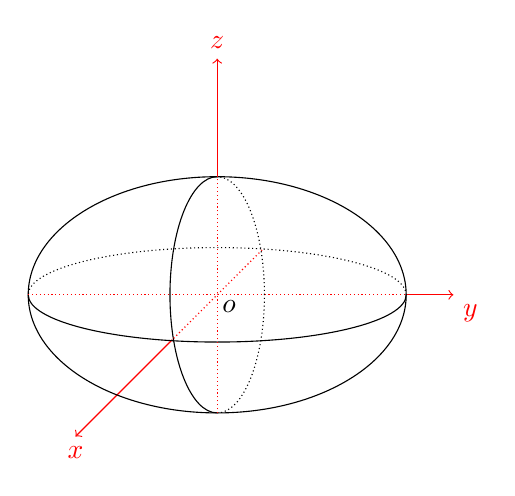
\begin{tikzpicture}[scale=3]
			\draw[red,->] (0.8,0) -- (1,0) node[anchor=north west]{$y$};
			\draw[red,->] (0,0.5) -- (0,1) node[anchor=south]{$z$};
			\draw[red,->] (-0.19,-0.19) -- (-0.6,-0.6) node[anchor=north]{$x$};
			\node at (0.05,-0.05) {$o$};
			\draw[densely dotted] (0.2,0) arc[start angle=0, end angle=90, x radius=0.2, y radius=0.5];
			\draw[densely dotted] (0,-0.5) arc[start angle=270, end angle=360, x radius=0.2, y radius=0.5];
			\draw (0,0.5) arc[start angle=90, end angle=270, x radius=0.2, y radius=0.5];
			\draw (0.8,0) arc[start angle=0, end angle=360, x radius=0.8, y radius=0.5];
			\draw[densely dotted] (0.8,0) arc[start angle=0, end angle=180, x radius=0.8, y radius=0.2];
			\draw (-0.8,0) arc[start angle=180, end angle=360, x radius=0.8, y radius=0.2];
			\draw[red,densely dotted] (-0.8,0) -- (0.8,0);
			\draw[red,densely dotted] (0,-0.5) -- (0,0.8);
			\draw[red,densely dotted] (0.19,0.19) -- (-0.19,-0.19);
		\end{tikzpicture}
		\caption{$\dfrac{x^{2}}{a^{2}} +\dfrac{y^{2}}{b^{2}}+\dfrac{z^{2}}{c^{2}}=1$}
	\end{figure}

	(b). 单叶双曲面 $\dfrac{x^{2}}{a^{2}} +\dfrac{y^{2}}{b^{2}} - \dfrac{z^{2}}{c^{2}}=1$

	\begin{figure}[H]
		\centering
		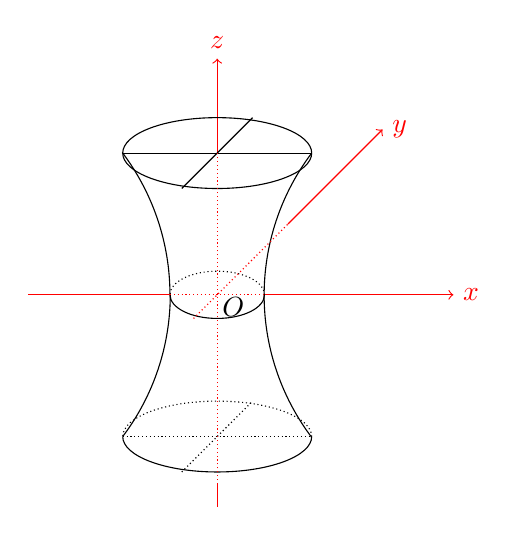
\begin{tikzpicture}[scale=3]
			\draw[red,->] (0.2,0) -- (1,0) node[right]{$x$};
			\draw[red,->] (0,0.6) -- (0,1) node[above]{$z$};
			\draw[red,->] (0.3,0.3) -- (0.7,0.7) node[right]{$y$};
			
			\draw (0.4,0.6) arc[start angle=0, end angle=360, x radius=0.4, y radius=0.15];
			\draw[densely dotted] (0.4,-0.6) arc[start angle=0, end angle=180, x radius=0.4, y radius=0.15];
			\draw (-0.4,-0.6) arc[start angle=180, end angle=360, x radius=0.4, y radius=0.15];
			
			\draw[densely dotted] (0.2,0) arc[start angle=0, end angle=180, x radius=0.2, y radius=0.1];
			\draw (-0.2,0) arc[start angle=180, end angle=360, x radius=0.2, y radius=0.1];
			
			\draw (0.4,0.6) arc[start angle=143, end angle=217, x radius=1, y radius=1];
			\draw (-0.4,-0.6) arc[start angle=323, end angle=360, x radius=1, y radius=1];
			\draw (-0.2,0) arc[start angle=0, end angle=37, x radius=1, y radius=1];
			
			\draw[red] (-0.8,0) -- (-0.2,0);
			\draw (-0.4,0.6) -- (0.4,0.6);
			\draw[red] (0,-0.8) -- (0,-0.9);
			\draw (-0.15,0.45) -- (0.15,0.75);
			\draw[densely dotted] (-0.4,-0.6) -- (0.4,-0.6);
			\draw[densely dotted] (-0.15,-0.75) -- (0.15,-0.45);
			\draw[red,densely dotted] (-0.2,0) -- (0.2,0);
			\draw[red,densely dotted] (0,-0.8) -- (0,0.6);
			\draw[red,densely dotted] (-0.1,-0.1) -- (0.3,0.3);
			\node at (-0.02,0.03) [below right] {$O$};
		\end{tikzpicture}
		\caption{$\dfrac{x^{2}}{a^{2}} +\dfrac{y^{2}}{b^{2}} - \dfrac{z^{2}}{c^{2}}=1$}
	\end{figure}

	(c). 双叶双曲面 $\dfrac{x^{2}}{a^{2}} - \dfrac{y^{2}}{b^{2}} - \dfrac{z^{2}}{c^{2}} = 1$

	\begin{figure}[H]
		\centering
		\begin{tikzpicture}[scale=3]
			\draw[red,->] (1.1,0) -- (1.4,0) node[right] {$x$};
			\draw[red,->] (0,-1.2) -- (0,1.2) node[above] {$z$}; 
			\draw[red,->] (-0.4,-0.5) -- (0.4,0.5) node[right] {$y$}; 
			
			\draw[densely dotted] (-0.9,0) arc[start angle=0, end angle=90, x radius=0.2, y radius=0.5];
			\draw[densely dotted] (-1.1,-0.5) arc[start angle=270, end angle=360, x radius=0.2, y radius=0.5];
			\draw (-1.1,0.5) arc[start angle=90, end angle=270, x radius=0.2, y radius=0.5];
			\draw (-0.4,0) arc[start angle=0, end angle=90, x radius=0.7, y radius=0.5];
			\draw (-1.1,-0.5) arc[start angle=270, end angle=360, x radius=0.7, y radius=0.5];
			\draw (-1.26,-0.25) arc[start angle=270, end angle=360, x radius=0.86, y radius=0.25];
			\draw[densely dotted] (-0.4,0) arc[start angle=0, end angle=90, x radius=0.54, y radius=0.25];
			\draw (1.3,0) arc[start angle=0, end angle=360, x radius=0.2, y radius=0.5];
			\draw (1.1,0.5) arc[start angle=90, end angle=270, x radius=0.7, y radius=0.5];
			\draw (0.4,0) arc[start angle=180, end angle=270, x radius=0.54, y radius=0.25];
			\draw[densely dotted] (1.26,0.25) arc[start angle=90, end angle=180, x radius=0.86, y radius=0.25];
			\draw[red] (-1.4,0) -- (-1.3,0);
			\draw[red] (-0.4,0) -- (0.4,0);
			\draw[densely dotted] (-1.1,0.5) -- (-1.1,-0.5);
			\draw[densely dotted] (-0.94,0.25) -- (-1.26,-0.25);
			\draw[red,densely dotted] (0.4,0) -- (1.1,0);
			\draw (0.94,-0.25) -- (1.26,0.25);
			\draw (1.1,0.5) -- (1.1,-0.5);
			\draw[red,densely dotted] (-1.3,0) -- (-0.4,0);
			\node at (0,0) [below right] {$O$};
		\end{tikzpicture}
		\caption{$\dfrac{x^{2}}{a^{2}} - \dfrac{y^{2}}{b^{2}} - \dfrac{z^{2}}{c^{2}} = 1$}
	\end{figure}

	(d). 椭圆抛物面 $\dfrac{x^{2}}{2p} + \dfrac{y^{2}}{2q} = z (p,q > 0)$

	\begin{figure}[H]
		\centering
		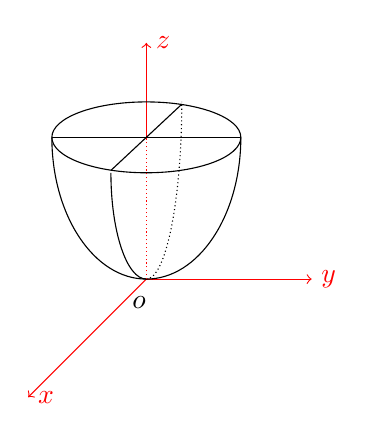
\begin{tikzpicture}[scale=3]
			\draw[red,->] (0,0) -- (-0.5,-0.5) node[right] {$x$};
			\draw[red,->] (0,0) -- (0.7,0) node[right] {$y$}; 
			\draw[red,->] (0,0.6) -- (0,1) node[right] {$z$}; 
			\draw (0.4,0.6) arc[start angle=0, end angle=360, x radius=0.4, y radius=0.15];
			\draw (-0.4,0.6) arc[start angle=180, end angle=360, x radius=0.4, y radius=0.6];
			\draw (-0.15,0.45) arc[start angle=180, end angle=270, x radius=0.15, y radius=0.45];
			\draw[densely dotted] (0,0) arc[start angle=270, end angle=360, x radius=0.15, y radius=0.75];
			\draw (-0.4,0.6) -- (0.4,0.6);
			\draw[red,densely dotted] (0,0) -- (0,0.6);
			\draw (-0.15,0.46) -- (0.15,0.74);
			\node at (-0.1,-0.1) [right] {$o$};
		\end{tikzpicture}
		\caption{$\dfrac{x^{2}}{2p} + \dfrac{y^{2}}{2q} = z (p,q > 0)$}
	\end{figure}
	
	(f). 椭圆锥面 $\dfrac{x^{2}}{a^{2}} + \dfrac{y^{2}}{b^{2}} = \dfrac{z^{2}}{c^{2}}$

	\begin{figure}[H]
		\centering
		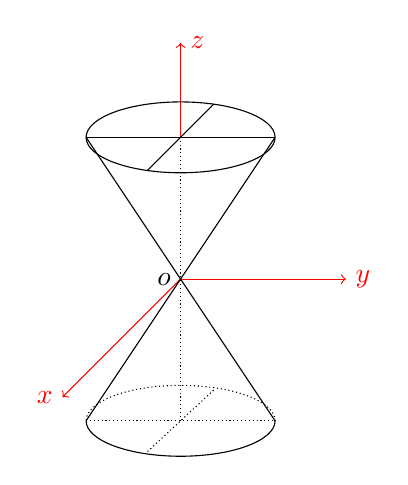
\begin{tikzpicture}[scale=3]
			\draw[red,->] (0,0) -- (-0.5,-0.5) node[left] {$x$};
			\draw[red,,->] (0,0) -- (0.7,0) node[right] {$y$}; 
			\draw[red,->] (0,0.6) -- (0,1) node[right] {$z$}; 
			\draw (0.4,0.6) arc[start angle=0, end angle=360, x radius=0.4, y radius=0.15];
			\draw[densely dotted] (0.4,-0.6) arc[start angle=0, end angle=180, x radius=0.4, y radius=0.15];
			\draw (-0.4,-0.6) arc[start angle=180, end angle=360, x radius=0.4, y radius=0.15];
			\draw (-0.4,0.6) -- (0.4,-0.6);
			\draw (0.4,0.6) -- (-0.4,-0.6);
			\draw (-0.4,0.6) -- (0.4,0.6);
			\draw[densely dotted] (-0.4,-0.6) -- (0.4,-0.6);
			\draw[densely dotted] (-0.14,-0.73) -- (0.14,-0.47);
			\draw[densely dotted] (0,-0.6) -- (0,0.6);
			\draw (-0.14,0.46) -- (0.14,0.74);
			\node at (0,0) [left] {$o$};
		\end{tikzpicture}
		\caption{$\dfrac{x^{2}}{a^{2}} + \dfrac{y^{2}}{b^{2}} = \dfrac{z^{2}}{c^{2}}$}
	\end{figure}

	(g). 双曲抛物面 $ - \dfrac{x^{2}}{2p} + \dfrac{y^{2}}{2q} = z (p,q > 0)$

	\begin{figure}[H]
		\centering
		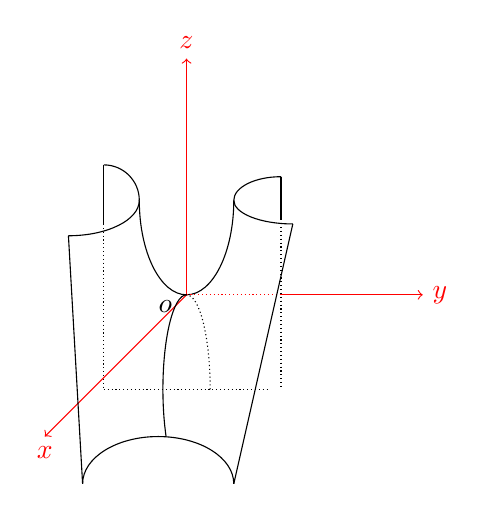
\begin{tikzpicture}[scale=3]
			\draw[red,->] (0.4,0) -- (1,0) node[right] {$y$};
			\draw[red,->] (0,0) -- (0,1) node[above] {$z$};
			\draw[red,->] (0,0) -- (-0.6,-0.6) node[below] {$x$};
			\draw (-0.2,0.4) arc[start angle=180, end angle=360, x radius=0.2, y radius=0.4];
			\draw (-0.2,0.4) arc[start angle=0, end angle=90, x radius=0.15, y radius=0.15];
			\draw (-0.5,0.25) arc[start angle=270, end angle=360, x radius=0.3, y radius=0.15];
			\draw (0.4,0.5) arc[start angle=90, end angle=180, x radius=0.2, y radius=0.1];
			\draw (0.2,0.4) arc[start angle=180, end angle=270, x radius=0.25, y radius=0.1];
			\draw (0.2,-0.8) arc[start angle=0, end angle=180, x radius=0.32, y radius=0.2];
			\draw[densely dotted] (0.1,-0.4) arc[start angle=0, end angle=90, x radius=0.1, y radius=0.4];
			\draw (0,0) arc[start angle=90, end angle=210, x radius=0.1, y radius=0.4];
			\draw[densely dotted] (-0.35,0.3) -- (-0.35,-0.4);
			\draw[densely dotted] (-0.35,-0.4) -- (0.35,-0.4);
			\draw[densely dotted] (0.4,0.5) -- (0.4,-0.4);
			\draw[red,densely dotted] (0,0) -- (0.4,0);
			\draw (0.4,0.5) -- (0.4,0.32);
			\draw (-0.35,0.55) -- (-0.35,0.3);
			\draw (-0.5,0.25) -- (-0.44,-0.8);
			\draw (0.45,0.3) -- (0.2,-0.8);
			\node at (-0.02, -0.05) [left]{$o$};
		\end{tikzpicture}
		\caption{$- \dfrac{x^{2}}{2p} + \dfrac{y^{2}}{2q} = z (p,q > 0)$}
	\end{figure}

	(h). 双曲抛物面 $z = xy$
	
	\begin{figure}[H]
		\centering
		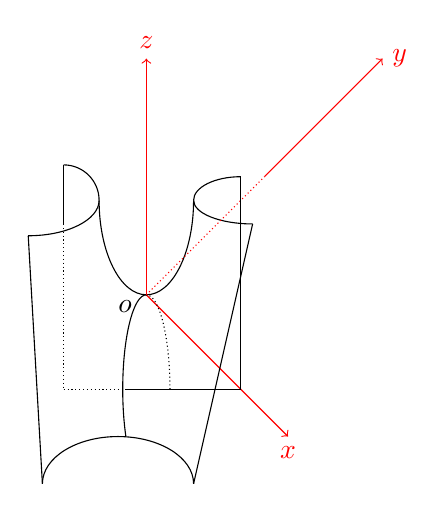
\begin{tikzpicture}[scale=3]
			\draw[red,->] (0.5,0.5) -- (1,1) node[right] {$y$};
			\draw[red,->] (0,0) -- (0,1) node[above] {$z$};
			\draw[red,->] (0,0) -- (0.6,-0.6) node[below] {$x$};
			\draw (-0.2,0.4) arc[start angle=180, end angle=360, x radius=0.2, y radius=0.4];
			\draw (-0.2,0.4) arc[start angle=0, end angle=90, x radius=0.15, y radius=0.15];
			\draw (-0.5,0.25) arc[start angle=270, end angle=360, x radius=0.3, y radius=0.15];
			\draw (0.4,0.5) arc[start angle=90, end angle=180, x radius=0.2, y radius=0.1];
			\draw (0.2,0.4) arc[start angle=180, end angle=270, x radius=0.25, y radius=0.1];
			\draw (0.2,-0.8) arc[start angle=0, end angle=180, x radius=0.32, y radius=0.2];
			\draw[densely dotted] (0.1,-0.4) arc[start angle=0, end angle=90, x radius=0.1, y radius=0.4];
			\draw (0,0) arc[start angle=90, end angle=210, x radius=0.1, y radius=0.4];
			\draw[densely dotted] (-0.35,0.3) -- (-0.35,-0.4);
			\draw[densely dotted] (-0.35,-0.4) -- (-0.09,-0.4);
			\draw (-0.09,-0.4) -- (0.4,-0.4);
			\draw (0.4,0.5) -- (0.4,-0.4);
			\draw[red,densely dotted] (0,0) -- (0.5,0.5);
			\draw (0.4,0.5) -- (0.4,0.32);
			\draw (-0.35,0.55) -- (-0.35,0.3);
			\draw (-0.5,0.25) -- (-0.44,-0.8);
			\draw (0.45,0.3) -- (0.2,-0.8);
			\node at (-0.02, -0.05) [left]{$o$};
		\end{tikzpicture}
		\caption{$z = xy$}
	\end{figure}

	(i). 椭圆柱面 $\dfrac{x^{2}}{a^{2}}+\dfrac{y^{2}}{b^{2}} = 1$
	
	\begin{figure}[H]
		\centering
		\begin{tikzpicture}[scale=3]
			\draw[red,->] (0,0.6) -- (0,1) node[right] {$z$};
			\draw[red,->] (0.3,0) -- (1,0) node[above] {$y$};
			\draw[red,->] (-0.1,-0.1) -- (-0.6,-0.6) node[below] {$x$};
			\draw (0.3,0.6) arc[start angle=0, end angle=360, x radius=0.3, y radius=0.1];
			\draw (-0.3,0) arc[start angle=180, end angle=360, x radius=0.3, y radius=0.1];
			\draw (-0.3,-0.4) arc[start angle=180, end angle=360, x radius=0.3, y radius=0.1];
			\draw[densely dotted] (0.3,0) arc[start angle=0, end angle=180, x radius=0.3, y radius=0.1];
			\draw[densely dotted] (0.3,-0.4) arc[start angle=0, end angle=180, x radius=0.3, y radius=0.1];
			\draw (-0.3,-0.4) -- (-0.3,0.6);
			\draw (0.3,-0.4) -- (0.3,0.6);
			\draw[red,densely dotted] (0,-0.5) -- (0,0.6);
			\draw[red,densely dotted] (-0.1,-0.1) -- (0.1,0.1);
			\draw[red,densely dotted] (-0.3,0) -- (0.3,0);
			\node at (0.1, -0.1) [below]{$o$};
		\end{tikzpicture}
		\caption{$\dfrac{x^{2}}{a^{2}}+\dfrac{y^{2}}{b^{2}} = 1$}
	\end{figure}
	

	(j). 双曲柱面 $\dfrac{x^{2}}{a^{2}} - \dfrac{y^{2}}{b^{2}} = 1$

	\begin{figure}[H]
		\centering
		\begin{tikzpicture}[scale=3]
			\draw[red,->] (0,0) -- (0,1) node[right] {$z$};
			\draw[red,->] (0,0) -- (1,0) node[above] {$x$};
			\draw[red,->] (-0.4,-0.4) -- (0.3,0.3) node[left] {\small{$y$}};
			\draw (0.8,0.6) arc[start angle=90, end angle=180, x radius=0.4, y radius=0.2];
			\draw (0.4,0.4) arc[start angle=180, end angle=270, x radius=0.1, y radius=0.1];
			\draw (-0.4,0.3) arc[start angle=0, end angle=90, x radius=0.1, y radius=0.1];
			\draw (-0.8,0.1) arc[start angle=270, end angle=360, x radius=0.4, y radius=0.2];
			\draw (-0.8,-0.25) arc[start angle=270, end angle=360, x radius=0.4, y radius=0.25];
			\draw (-0.8,-0.6) arc[start angle=270, end angle=360, x radius=0.4, y radius=0.25];
			\draw[densely dotted] (-0.4,-0.35) arc[start angle=0, end angle=90, x radius=0.1, y radius=0.1];
			\draw[densely dotted] (-0.4,0) arc[start angle=0, end angle=90, x radius=0.1, y radius=0.1];
			\draw (0.4,0) arc[start angle=180, end angle=270, x radius=0.1, y radius=0.1];
			\draw (0.4,-0.4) arc[start angle=180, end angle=270, x radius=0.1, y radius=0.1];
			\draw[densely dotted] (0.8,0.3) arc[start angle=90, end angle=180, x radius=0.4, y radius=0.3];
			\draw[densely dotted] (0.8,-0.1) arc[start angle=90, end angle=180, x radius=0.4, y radius=0.3];
			\draw[densely dotted] (-0.5,-0.25) -- (-0.5,0.16);
			\draw[red,densely dotted] (-0.7,0) -- (-0.4,0);
			\draw[red] (-0.4,0) -- (0,0);
			\draw (-0.5,0.16) -- (-0.5,0.4);
			\draw (0.4,-0.4) -- (0.4,0.4);
			\draw (0.8,-0.1) -- (0.8,0.6);
			\draw (-0.4,0.3) -- (-0.4,-0.4);
			\draw (-0.8,0.1) -- (-0.8,-0.6);
			\draw (0.5,-0.5) -- (0.5,0.3);
			\node at (0.1, -0.1) [below]{$o$};
		\end{tikzpicture}
		\caption{$\dfrac{x^{2}}{a^{2}} - \dfrac{y^{2}}{b^{2}} = 1$}
	\end{figure}
	

	(k). 抛物柱面 $ y = ax^{2}$

	\begin{figure}[H]
		\centering
		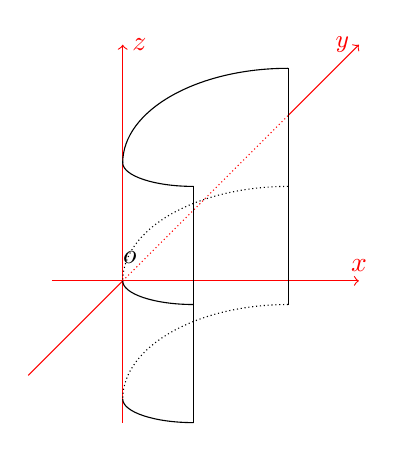
\begin{tikzpicture}[scale=3]
			\draw[red,->] (0,-0.6) -- (0,1) node[right] {$z$};
			\draw[red,->] (-0.3,0) -- (1,0) node[above] {$x$};
			\draw[red,->] (0.7,0.7) -- (1,1) node[left] {\small{$y$}};
			\draw[red,densely dotted] (0,0) -- (0.7,0.7);
			\draw[red] (-0.4,-0.4) -- (0,0);
			\draw (0.7,0.9) arc[start angle=90, end angle=180, x radius=0.7, y radius=0.4];
			\draw (0,0.5) arc[start angle=180, end angle=270, x radius=0.3, y radius=0.1];
			\draw (0,0) arc[start angle=180, end angle=270, x radius=0.3, y radius=0.1];
			\draw (0,-0.5) arc[start angle=180, end angle=270, x radius=0.3, y radius=0.1];
			\draw[densely dotted] (0.7,0.4) arc[start angle=90, end angle=180, x radius=0.7, y radius=0.4];
			\draw[densely dotted] (0.7,-0.1) arc[start angle=90, end angle=180, x radius=0.7, y radius=0.4];
			\draw (0.3,0.4) -- (0.3,-0.6);
			\draw (0.7,-0.1) -- (0.7,0.9);
			\node at (0.1, 0.1) [left]{$o$};
		\end{tikzpicture}
		\caption{$y = ax^{2}$}
	\end{figure}

	(3). 旋转曲面

	曲线 $\Gamma : \begin{cases}
	  F(x,y,z) = 0\\
	  G(x,y,z) = 0
	\end{cases}$ 绕直线 $L: \dfrac{x-x_{0}}{l} = \dfrac{y-y_{0}}{m} = \dfrac{z-z_{0}}{n}$ 旋转一周形成的旋转曲面, 直线 $L$ 的方向向量 
	$\boldsymbol{\tau} = (l,m,n)$

	设 $M_{1}(x_{1},y_{1},z_{1})$ 是曲线 $\Gamma$ 上任意一点, $P(x,y,z)$ 是 $M_{1}$ 绕直线 $L$ 旋转一周形成的纬圆上异于 $M_{1}$ 的一点:
	$$\begin{cases}
	  \boldsymbol{\tau} \perp \overrightarrow{M_{1}P} \\
	  |\overrightarrow{M_{1}M_{0}}| = |\overrightarrow{PM_{0}}|\\
	  F(x_{1},y_{1},z_{1}) = 0\\
	  G(x_{1},y_{1},z_{1}) = 0
	\end{cases}$$
\end{definition}
\subsection{空间曲线的切线和法平面}
\begin{definition}[曲线切线和法平面]
	
	(1).参数方程
	$$\begin{cases}
		x = f(t)\\
		y = g(t)\\
		z = h(t)
	\end{cases}, t \in [\alpha,\beta]$$
	
	在 $t=t_{0}$ 时,点 $P_{0}(x(t_{0}),y(t_{0}),z(t_{0}))$ 处切线的方向向量 $\boldsymbol{n}=(f'(t_{0}),g'(t_{0}),h'(t_{0}))$
	
	\textcolor{cyan}{切线方程}
	
	$$\dfrac{x-x_{0}}{f'(t_{0})}=\dfrac{y-y_{0}}{g'(t_{0})}=\dfrac{z-z_{0}}{h'(t_{0})}$$
	
	\textcolor{purplea}{法平面方程}
	
	$$f'(t_{0})(x-x_{0})+g'(t_{0})(y-y_{0})+h'(t_{0})(z-z_{0})=0$$
	
	(2). 一般式
	$$\begin{cases}
		F(x,y,z) = 0\\
		G(x,y,z) = 0
	\end{cases}$$
	
	点 $P_{0}(x_{0},y_{0},z_{0})$ 处切线的方向向量
	$$\boldsymbol{\tau} = 
	\begin{vmatrix}
	  \boldsymbol{i} & \boldsymbol{j} & \boldsymbol{k}\\
	  F_{x}' & F_{y}' & F_{z}'\\
	  G_{x}' & G_{y}' & G_{z}'
	\end{vmatrix} = (A,B,C)$$

	
	\textcolor{cyan}{切线方程}
	
	$$\dfrac{x-x_{0}}{A} = \dfrac{y-y_{0}}{B} = \dfrac{z-z_{0}}{C}$$
	
	\textcolor{purplea}{法平面方程}
	
	$$A(x-x_{0}) + B(y-y_{0}) + C(z-z_{0}) = 0$$
	
	
\end{definition}

\subsection{空间曲面的切平面和法线}
\begin{definition}
	
	(1). $F(x,y,z)=0$, 点 $P(x_{0},y_{0},z_{0})$ 处切平面法向量 $\boldsymbol{n} = \{F_{x}'(x_{0},y_{0},z_{0}),F_{y}'(x_{0},y_{0},z_{0}),F_{z}'(x_{0},y_{0},z_{0})\}$
	
	\textcolor{cyan}{切平面方程}
	
	$$F_{x}'(x_{0},y_{0},z_{0})(x-x_{0}) + F_{y}'(x_{0},y_{0},z_{0})(y-y_{0}) + F_{z}'(x_{0},y_{0},z_{0})(z-z_{0}) = 0$$

	\textcolor{purplea}{法线方程}
	
	$$\dfrac{x-x_{0}}{F_{x}'(x_{0},y_{0},z_{0})} = \dfrac{y-y_{0}}{F_{y}'(x_{0},y_{0},z_{0})}=\dfrac{z-z_{0}}{F_{z}'(x_{0},y_{0},z_{0})}$$
	
	(2). $z=f(x,y)$, 点 $P(x_{0},y_{0},z_{0})$ 处切平面法向量 $\boldsymbol{n} = \{f_{x}'(x_{0},y_{0}),f_{y}'(x_{0},y_{0}),-1\}$
	
	
	\textcolor{cyan}{切平面方程}

	$$f_{x}'(x_{0},y_{0})(x-x_{0}) + f_{y}'(x_{0},y_{0})(y-y_{0}) - (z-z_{0}) = 0$$
	
	\textcolor{purplea}{法线方程}
	
	$$\dfrac{x-x_{0}}{f_{x}'(x_{0},y_{0})} = \dfrac{y-y_{0}}{f_{y}'(x_{0},y_{0})} = \dfrac{z-z_{0}}{-1}$$
\end{definition}

\section{场论初步}

\subsection{方向导数}
\begin{definition}[方向导数]
	
	设三元函数 $u=u(x,y,z)$ 在点 $P(x_{0},y_{0},z_{0})$ 的某空间邻域内 $U\subset R^3$ 有定义,$l$ 是从 $P_{0}$ 出发的一条射线,$P(x,y,z)$ 为 $l$ 上且在 $U$ 中的任意一点: 
	$$\begin{cases}
		x-x_{0}=\Delta x=t\cos \alpha\\
		y-y_{0}=\Delta y=t\cos \beta\\
		z-z_{0}=\Delta z=t\cos \gamma
	\end{cases}$$ 
	
	$t=\sqrt{(\Delta x)^2+(\Delta y)^2+(\Delta z)^2}$ 表示 $|PP_{0}|$,如果下面极限存在: 

	$$\lim\lim\limits_{t\to 0}\frac{u(P)-u(P_{0})}{t}=\lim\lim\limits_{t\to 0}\frac{u(x_{0}+t\cos \alpha,y_{0}+t\cos \beta,z_{0}+t\cos \gamma)-u(x_{0},y_{0},z_{0})}{t}$$
	
	我们将此极限称为 $u=f(x,y,z)$ 在$P_{0}$ 处沿着 $l$ 的方向导数,记作 $\dfrac{\partial u}{\partial l}|_{P_{0}}$
\end{definition}

\begin{theorem}[方向导数计算公式]
	$$\dfrac{\partial u}{\partial \boldsymbol{l}}|_{P_{0}}=u_{x}'\cos \alpha+u_{y}'\cos \beta+u_{z}'\cos \gamma$$
	
	其中$\cos \alpha,\cos \beta,\cos \gamma$ 为方向 $\boldsymbol{l}$ 的方向余弦
\end{theorem}

\subsection{梯度}

\begin{definition}[梯度]
	
	设三元函数 $u=u(x,y,z)$ 在点 $P(x_{0},y_{0},z_{0})$ 处具有一阶偏导数,定义下面为 $u=u(x,y,z)$ 在 $ P_{0}(x_{0},y_{0},z_{0})$ 处的梯度: 
	
	$$\boldsymbol{guad}\ u|_{P_{0}}=(u_{x}'(P_{0}),u_{y}'(P_{0}),u_{z}'(P_{0}))$$
	
	
	梯度和方向导数之间的关系: 

	$$\dfrac{\partial u}{\partial l}|_{P_{0}}=\boldsymbol{guad}\ u|_{P_{0}}\cdot \boldsymbol{l}=\big|\boldsymbol{guad}\ u|_{P_{0}}\big| |l|\cos \theta$$
\end{definition}

\subsection{散度和旋度}

\begin{definition}[散度和旋度]
	设向量场 $\boldsymbol{A}(x,y,z)=P(x,y,z)\boldsymbol{i} + Q(x,y,z)\boldsymbol{j} + R(x,y,z)\boldsymbol{k}$
	
	\textcolor{cyan}{散度} 
	$$div\ \boldsymbol{A}=\dfrac{\partial P}{\partial x}+\dfrac{\partial Q}{\partial y}+\dfrac{\partial R}{\partial z}$$
	
	\textcolor{purplea}{旋度}
	$$rot \ \boldsymbol{A} = 
	\begin{vmatrix}
		\boldsymbol{i} & \boldsymbol{j} & \boldsymbol{k}\\
		\dfrac{\partial}{\partial x} & \dfrac{\partial}{\partial y} & \dfrac{\partial}{\partial z} \\
		P & Q & R
	\end{vmatrix}$$
\end{definition}



\chapterimage{chap12.jpg}
\chapter{三重积分(非数二)}

\section{三重积分定义和性质}

\begin{definition}[三重积分]
	设 $f(x, y, z)$ 是空间有界闭区域 $\Omega$ 上的有界函数, 将 $\Omega$ 任意分为 $n$ 个小闭区域
	$$\Delta v_{1}, \Delta v_{2}, \cdots, \Delta v_{n}$$
	其中 $\Delta v_{i}$ 表示第 $i$ 个小闭区域, 也表示第 $i$ 个小闭区域的体积, 在每一个 $\Delta v_{i}$ 中任意取一点 $(\xi_{i}, \eta_{i}, \zeta_{i})$, 作乘积 $f(\xi_{i},\eta_{i},\zeta_{i})\Delta v_{i}(i = 1,2,\cdots,n)$,
	并求和 $\sum_{i=1}^{n}f(\xi_{i},\eta_{i},\zeta_{i})\Delta v_{i}$, 如果当 $\lim\limits_{n \to +\infty}\{\lambda |\lambda = \max\{\Delta v_{i}\text{的直径}, i = 1,2,\cdots,n\}\} = 0$ 时, 求和的极限总是存在, 
	与 $\Delta v_{i}$ 的分法以及点 $(\xi_{i}, \eta_{i}, \zeta_{i})$ 的选取无关, 称此极限为函数 $f(x,y,z)$ 在闭区域 $\Omega$ 上的三重积分, 记作 $\iiint\limits_{\Omega}f(x,y,z)dv$

	$$\iiint\limits_{\Omega}f(x,y,z)dv = \lim\limits_{\lambda \to 0}\sum_{i=1}^{n}f(\xi_{i},\eta_{i},\zeta_{i})\Delta v_{i}$$
	
	其中 $f(x,y,z)$ 称为被积函数, $\Omega$ 称为积分区域, $f(x,y,z)dv$ 称为被积表达式, $dv$ 称为体积微元, $x,y,z$ 称为积分变量, $\sum\limits_{i=1}^{n} f(\xi_{i},\eta_{i},\zeta_{i})\Delta v_{i}$ 称为积分和

	\textcolor{cyan}{物理意义}

	设一物体占有 $Oxyz$ 上闭区域 $\Omega$, 在点 $(x,y,z)$ 处的密度为 $\rho(x,y,z)$, 假定 $\rho(x,y,z)$ 在 $\Omega$ 上连续, 物体质量 $M = \iiint\limits_{\Omega}\rho(x,y,z)dv$
\end{definition}

\begin{corollary}

	(1). 当 $f(x,y,z)$ 在闭区域 $\Omega$ 上连续时, 三重积分 $\iiint\limits_{\Omega}f(x,y,z)dv$ 一定存在; 当 $f(x,y,z)$ 在 $\Omega$ 上可积, $f(x,y,z)$ 在 $\Omega$ 上必有界

	(2). $\iint\limits_{\Omega}1dv = \iiint\limits_{\Omega}dv = V$, $V$ 是 $\Omega$ 的体积

	(3). 积分线性性质

	$$\iiint\limits_{\Omega}\left[k_{1}f(x,y,z)\pm k_{2}g(x,y,z)\right] dv=k_{1}\iiint\limits_{\Omega}f(x,y,z)dv \pm k_{2}\iiint\limits_{\Omega}g(x,y,z)dv$$
	
	(4). 积分的可加性

	设 $f(x,y,z)$ 在 $\Omega$ 上可积, 且 $\Omega_{1} \cap \Omega_{2} = \emptyset, \Omega_{1} \cup \Omega_{2} =\Omega$
	$$\iiint\limits_{\Omega}f(x,y,z)dv = \iiint\limits_{\Omega_{1}}f(x,y,z)dv + \iiint\limits_{\Omega_{2}}f(x,y,z)dv $$

	(5). 积分保号性

	设 $f(x,y,z)$ 和 $g(x,y,z)$ 在 $\Omega$ 上可积, 且在 $\Omega$ 上, $f(x,y,z)\leq g(x,y,z)$

	$$\iiint\limits_{\Omega}f(x,y,z)dv \leq \iiint\limits_{\Omega}g(x,y,z)dv \Rightarrow \big|\iiint\limits_{\Omega}f(x,y,z)dv\big| \leq \iiint\limits_{\Omega}\big|f(x,y,z)\big|dv$$

	(6). 估值定理

	设 $M,m$ 分别是 $f(x,y,z)$ 在 $\Omega$ 上的最大值和最小值, $V$ 是 $\Omega$ 的体积
	
	$$mV \leq \iiint\limits_{\Omega}f(x,y,z)dv \leq MV$$

	(7). 中值定理

	设 $f(x,y,z)$ 在 $\Omega$ 上连续, $V$ 是 $\Omega$ 的体积

	$$\exists (\xi,\eta,\zeta) \in \Omega,\ s.t.\ \iiint\limits_{\Omega}f(x,y,z)dv = f(\xi,\eta,\zeta)V $$

\end{corollary}

\section{三重积分对称性}

\begin{definition}[普通对称性]
	(1). $\Omega$ 关于平面 $xoz$ 对称

	$$\iiint\limits_{\Omega}f(x,y,z)dv = 
	\begin{cases}
		2\iiint\limits_{\Omega_{1}}f(x,y,z)dv & f(x,y,z) = f(x,-y,z)\\
		0                                     & f(x,y,z) = -f(x,-y,z)
	\end{cases}$$

	(2). $\Omega$ 关于平面 $yoz$ 对称

	$$\iiint\limits_{\Omega}f(x,y,z)dv =
	\begin{cases}
		2\iiint\limits_{\Omega_{1}}f(x,y,z)dv & f(x,y,z) = f(-x,y,z)\\
		0                                     & f(x,y,z) = -f(-x,y,z)
	\end{cases}$$

	(3). $\Omega$ 关于平面 $xoy$ 对称

	$$\iiint\limits_{\Omega}f(x,y,z)dv =
	\begin{cases}
		2\iiint\limits_{\Omega_{1}}f(x,y,z)dv & f(x,y,z) = f(x,y,-z)\\
		0                                     & f(x,y,z) = -f(x,y,-z)
	\end{cases}$$

\end{definition}

\begin{definition}[轮换对称性]
	若将 $x,y,z$ 任意两个交换位置后, 积分区域 $\Omega$ 保持不变

	$$\iiint\limits_{\Omega}f(x)dv=\iiint\limits_{\Omega}f(y)dv=\iiint\limits_{\Omega}f(z)dv$$
\end{definition}

\section{三重积分计算方法}


\begin{definition}[直角坐标系]
	(1). \textcolor{cyan}{先一后二}

	$$\iiint\limits_{\Omega}f(x,y,z)dv=\iint\limits_{D_{xy}}d\sigma \int_{z_{1}(x,y)}^{z_{2}(x,y)}f(x,y,z)dz$$
	
	一般用于空间区域 $\Omega$ 无侧面或者侧面为柱面, 转化为二重积分, 积分区域为空间区域 $\Omega$ 在 $xoy(yoz,xoz)$ 平面的投影
	
	(2). \textcolor{cyan}{先二后一}

	$$\iiint\limits_{\Omega}f(x,y,z)dv = \int_{a}^{b}dz\iint\limits_{D_{z}}f(x,y,z)d\sigma$$
	
	适用于旋转体, 旋转曲面方程 $z = z(x,y)$
\end{definition}

\begin{definition}[换元法]
	令 $\begin{cases}
	   x = x(u,v,w) \\
	   y = y(u,v,w) \\
	   z = z(u,v,w)
	\end{cases}$, 且 $(x,y,z)\to (u,v,w)$ 是一一映射, $x = x(u,v,w), y = y(u,v,w), z = z(u,v,w)$ 有一阶连续偏导数
	$$\begin{vmatrix}
		\dfrac{\partial (x,y,z)}{\partial (u,v,w)}
	  \end{vmatrix} = 
	\begin{Vmatrix}
	  \dfrac{\partial x}{\partial u} & \dfrac{\partial x}{\partial v} & \dfrac{\partial x}{\partial w} \\
	  \dfrac{\partial y}{\partial u} & \dfrac{\partial y}{\partial v} & \dfrac{\partial y}{\partial w} \\
	  \dfrac{\partial z}{\partial u} & \dfrac{\partial z}{\partial v} & \dfrac{\partial z}{\partial w}
	\end{Vmatrix}\neq 0$$

	$$\iiint\limits_{\Omega_{xyz}}f(x,y,z)dxdydz = \iiint\limits_{\Omega_{uvw}}f \left[x(u,v,w), y(u,v,w), z(u,v,w)\right] 
	\begin{vmatrix}
	  \dfrac{\partial (x,y,z)}{\partial (u,v,w)}
	\end{vmatrix}
	dudvdw$$
\end{definition}

\begin{definition}[柱面坐标系]
	令 $\begin{cases}
	  x = r\cos \theta, & \theta\in [0,2\pi] \\
	  y = r\sin \theta, & \theta\in [0,2\pi] \\
	  z = z
	\end{cases}$, 且 $(x,y,z)\to (r,\theta,z)$ 是一一映射, $x = r\cos \theta, y = r\sin \theta, z = z$ 有一阶连续偏导数
	
	$$\begin{vmatrix}
		\dfrac{\partial (x,y,z)}{\partial (r,\theta,z)}
	  \end{vmatrix} = 
	\begin{Vmatrix}
	  \dfrac{\partial x}{\partial r} & \dfrac{\partial x}{\partial \theta} & \dfrac{\partial x}{\partial z} \\
	  \dfrac{\partial y}{\partial r} & \dfrac{\partial y}{\partial \theta} & \dfrac{\partial y}{\partial z} \\
	  \dfrac{\partial z}{\partial r} & \dfrac{\partial z}{\partial \theta} & \dfrac{\partial z}{\partial z}
	\end{Vmatrix} = 
	\begin{Vmatrix}
	  \cos \theta & -r\sin \theta & 0 \\
	  \sin \theta & r\cos \theta & 0 \\
	  0 & 0 & 1
	\end{Vmatrix} = r$$
	
	$$\iiint\limits_{\Omega_{xyz}}f(x,y,z)dxdydz=\iint\limits_{\Omega_{r\theta z}}drd\theta \int_{z_{1}(r,\theta)}^{z_{2}(r,\theta)}rf(r\cos \theta,r\sin\theta,z)dz$$
\end{definition}

\begin{definition}[球面坐标系]
	令 $\begin{cases}
		x = r\sin\varphi\cos\theta, & \theta\in [0,2\pi]\\
		y = r\sin\varphi\sin\theta, & \theta\in [0,2\pi]\\\
		z = r\cos\varphi, & \varphi\in [0,\pi]
	\end{cases}$, 且 $(x,y,z) \to (r,\theta,\varphi)$ 是一一映射, $x = r\sin\varphi\cos\theta, y = r\sin\varphi\sin\theta, z = r\cos\varphi$ 有一阶连续偏导数

	$$\begin{vmatrix}
		\dfrac{\partial (x,y,z)}{\partial (r,\theta,\varphi)}
	\end{vmatrix} = 
	\begin{Vmatrix}
	  \dfrac{\partial x}{\partial r} & \dfrac{\partial x}{\partial \theta} & \dfrac{\partial x}{\partial \varphi} \\
	  \dfrac{\partial y}{\partial r} & \dfrac{\partial y}{\partial \theta} & \dfrac{\partial y}{\partial \varphi} \\
	  \dfrac{\partial z}{\partial r} & \dfrac{\partial z}{\partial \theta} & \dfrac{\partial z}{\partial \varphi}
	\end{Vmatrix} = 
	\begin{Vmatrix}
	  \sin\varphi\sin\theta & -r\sin\varphi\sin\theta & r\cos\varphi\cos\theta \\
	  \cos\varphi\cos\theta & r\sin\varphi\cos\theta & r\cos\varphi\sin\theta \\
	  \cos\varphi & 0 & -r\sin \varphi
	\end{Vmatrix} = r^{2}\sin\varphi$$

	$$\iiint\limits_{\Omega_{xyz}}f(x,y,z)dxdydz=\iiint\limits_{\Omega_{r\varphi\theta}}r^2\sin\varphi f(r\sin\varphi\cos\theta,r\sin\varphi\sin\theta,r\cos\varphi) drd\theta d\varphi$$
\end{definition}

\section{三重积分应用}
\begin{theorem}[重心公式]

	对于空间物体, 体密度 $\rho(x,y,z)$, $\Omega$ 是物体所占的空间区域, 重心 $O(\overline{x}, \overline{y}, \overline{z})$
	$$\begin{cases}
		\overline{x} = \dfrac{\iiint\limits_{\Omega}x\rho(x,y,z)dv}{\iiint\limits_{\Omega}\rho(x,y,z)dv} \\
		\overline{y} = \dfrac{\iiint\limits_{\Omega}y\rho(x,y,z)dv}{\iiint\limits_{\Omega}\rho(x,y,z)dv} \\
		\overline{z} = \dfrac{\iiint\limits_{\Omega}z\rho(x,y,z)dv}{\iiint\limits_{\Omega}\rho(x,y,z)dv}
	\end{cases}$$
	
	当密度函数为 $\rho(x,y,z)$ 为常数, 重心就是形心

	$$\begin{cases}
		\overline{x} = \dfrac{\iiint\limits_{\Omega}xdv}{\iiint\limits_{\Omega}dv} \\
		\overline{y} = \dfrac{\iiint\limits_{\Omega}ydv}{\iiint\limits_{\Omega}dv} \\
		\overline{z} = \dfrac{\iiint\limits_{\Omega}zdv}{\iiint\limits_{\Omega}dv}
	\end{cases}\Rightarrow 
	\begin{cases}
		\iiint\limits_{\Omega}xdv = \overline{x}\cdot V\\
		\iiint\limits_{\Omega}ydv = \overline{y}\cdot V\\
		\iiint\limits_{\Omega}zdv = \overline{z}\cdot V
	\end{cases}$$
\end{theorem}

\begin{theorem}[转动惯量 $I = \sum\limits_{i=1}^{n}m_{i}r_{i}^{2}$]

	对于空间物体, 体密度 $\rho(x,y,z)$, $\Omega$ 是物体所占的空间区域

	(1). $x$ 轴
	$$I_{x} = \iint\limits_{\Omega}(y^{2}+z^{2})\rho(x,y,z)dv$$

	(2). $y$ 轴

	$$I_{y} = \iint\limits_{\Omega}(x^{2}+z^{2})\rho(x,y,z)dv$$

	(3). $z$ 轴

	$$I_{z} = \iint\limits_{\Omega}(x^{2}+y^{2})\rho(x,y,z)dv$$

	(4). 原点 $O$

	$$I_{O} = \iint\limits_{\Omega}(x^{2}+y^{2}+z^{2})\rho(x,y,z)dv$$
\end{theorem}

\begin{theorem}[万有引力 $F = G\frac{m_{1}m_{2}}{r^{2}}$]

	对于空间物体, 体密度 $\rho(x,y,z)$, $\Omega$ 是物体所占的空间区域, 计算该物体对物体外一点 $M_{0}(x_{0},y_{0},z_{0})$ 处质量为 $m$ 的质点的引力 $\boldsymbol{F} = (F_{x},F_{y},F_{z})$
	
	\begin{eqnarray*}
		F_{x} & = & Gm \iiint\limits_{\Omega}\dfrac{\rho(x,y,z)}{(x-x_{0})^{2}+(y-y_{0})^{2}+(z-z_{0})^{2}}\cos\alpha dv \\
		      & = & Gm \iiint\limits_{\Omega}\dfrac{\rho(x,y,z)(x-x_{0})}{\left[(x-x_{0})^{2}+(y-y_{0})^{2}+(z-z_{0})^{2}\right]^{\frac{3}{2}}}
	\end{eqnarray*}

	\begin{eqnarray*}
		F_{y} & = & Gm \iiint\limits_{\Omega}\dfrac{\rho(x,y,z)}{(y-y_{0})^{2}+(y-y_{0})^{2}+(z-z_{0})^{2}}\cos\beta dv \\
		      & = & Gm \iiint\limits_{\Omega}\dfrac{\rho(x,y,z)(y-y_{0})}{\left[(x-x_{0})^{2}+(y-y_{0})^{2}+(z-z_{0})^{2}\right]^{\frac{3}{2}}}
	\end{eqnarray*}

	\begin{eqnarray*}
		F_{z} & = & Gm \iiint\limits_{\Omega}\dfrac{\rho(x,y,z)}{(z-z_{0})^{2}+(y-y_{0})^{2}+(z-z_{0})^{2}}\cos\gamma dv \\
		      & = & Gm \iiint\limits_{\Omega}\dfrac{\rho(x,y,z)(z-z_{0})}{\left[(x-x_{0})^{2}+(y-y_{0})^{2}+(z-z_{0})^{2}\right]^{\frac{3}{2}}}
	\end{eqnarray*}
\end{theorem}


\chapterimage{chap13.jpg}
\chapter{第一型曲线和曲面积分}

\section{第一型曲线积分}

\subsection{第一型曲线积分定义和性质}

\begin{definition}[第一型曲线积分]
	设 $L$ 是 $xoy$ 平面内一条光滑曲线弧, 函数 $f(x,y)$ 在 $L$ 上有界, 在 $L$ 上任意插入一系列的点 $M_{1}, M_{2}, \cdots, M_{n-1}$ 将 $L$ 分成 $n$ 小段, 设第 $i$ 段的弧长为 $\Delta s_{i}$, 
	在 第 $i$ 段上任意取一点 $(\zeta_{i},\eta_{i})$, 作乘积 $f(\zeta_{i},\eta_{i})\Delta s_{i}(i=1,2,\cdots,n)$, 并求和 $\sum\limits_{i=1}^{n}f(\zeta_{i},\eta_{i})\Delta s_{i}$, 当 
	$\lim\limits_{n \to +\infty}\{\lambda|\lambda = \max\{\Delta s_{i}\}, i =1,2,\cdots,n\} = 0$ 时, 求和极限存在, 
	且与 $\Delta s_{i}$ 的分法以及 $(\zeta_{i},\eta_{i})$ 的取法无关, 称此极限为函数 $f(x,y)$ 在曲线 $L$ 上对弧长的曲线积分
	或第一型曲线积分, 记作 $\int_{L}f(x,y)ds$
	$$\int_{L}f(x,y)ds = \lim\limits_{\lambda \to 0}\sum\limits_{i=1}^{n}f(\zeta_{i},\eta_{i})\Delta s_{i}$$ 

	其中 $f(x,y)$ 称为被积函数, $f(x,y)ds$ 称为被积表达式, $x,y$ 是积分变量, $L$ 是积分弧

	对于函数 $f(x,y,z)$ 在空间曲线 $\Gamma$ 上的第一型曲线积分
	$$\int_{\Gamma}f(x,y,z)ds = \lim\limits_{\lambda \to 0}\sum\limits_{i=1}^{n}f(\xi_{i},\eta_{i},\zeta_{i})\Delta s_{i}$$

	\textcolor{cyan}{物理意义}

	1. 设一物体在 $xoy$ 平面内一光滑曲线弧 $L$ 上, 物体在 $L$ 上的线密度为 $\rho(x,y)$, 则物体的质量 $m = \int_{L}\rho(x,y)ds$

	2. 设一物体在空间曲线 $\Gamma$ 上, 物体在 $\Gamma$ 上的线密度为 $\rho(x,y,z)$, 则物体的质量 $m = \int_{\Gamma}\rho(x,y,z)ds$
\end{definition}
\begin{corollary}

	(1). $\displaystyle{\int_{\Gamma} ds = l_{\Gamma}}$, 其中 $l_{\Gamma}$ 是 $\Gamma$ 的长度

	(2). 设 $f(x,y,z)$ 在 $\Gamma$ 上可积, 其在 $\Gamma$ 上必有界

	(3). 积分线性性质
	$$\int_{\Gamma}\left[k_{1}f(x,y,z) + k_{2} g(x,y,z)\right]ds = k_{1}\int_{\Gamma}f(x,y,z)ds+k_{2}\int_{\Gamma}g(x,y,z)ds$$

	(4). 积分可加性

	设 $f(x,y,z)$ 在 $\Gamma$ 上可积, 且 $\Gamma_{1}\cap \Gamma_{2}=\emptyset, \Gamma_{1}\cup \Gamma_{2}=\Gamma$

	$$\int_{\Gamma}f(x,y,z)ds = \int_{\Gamma_{1}}f(x,y,z)ds + \int_{\Gamma_{2}}f(x,y,z)ds$$

	(5). 积分保号性

	设 $f(x,y,z), g(x,y,z)$ 在 $\Gamma$ 上可积, 且在 $\Gamma$ 上 $f(x,y,z) \leq g(x,y,z)$
	$$\int_{\Gamma}f(x,y,z)ds \leq \int_{\Gamma}g(x,y,z)ds\Rightarrow \big|\int_{\Gamma}f(x,y,z)ds\big| \leq \int_{\Gamma}\big|f(x,y,z)\big|ds$$

	(6). 估值定理
	设 $M,m$ 分别是 $f(x,y,z)$ 在 $\Gamma$ 上的最大值和最小值, $l_{\Gamma}$ 的长度
	$$ml_{\Gamma} \leq \int_{\Gamma}f(x,y,z)ds \leq Ml_{\Gamma}$$

	(7). 中值定理

	设 $f(x,y,z)$ 在 $\Gamma$ 上连续, $l_{\Gamma}$ 是 $\Gamma$ 的长度

	$$\exists (\xi,\eta,\zeta)\in \Gamma,\ s.t.\ \int_{\Gamma}f(x,y,z) ds = f(\xi,\eta,\zeta)l_{\Gamma}$$
\end{corollary}

\subsection{第一型曲线积分的对称性}

\begin{definition}[普通对称性]
	(1). $\Gamma$ 关于平面 $xoz$ 对称

	$$\int_{\Gamma}f(x,y,z)ds = 
	\begin{cases}
		2\int_{\Gamma_{1}}f(x,y,z)ds & f(x,y,z) = f(x,-y,z)\\
		0                                     & f(x,y,z) = -f(x,-y,z)
	\end{cases}$$

	(2). $\Gamma$ 关于平面 $yoz$ 对称

	$$\int_{\Gamma}f(x,y,z)ds =
	\begin{cases}
		2\int_{\Gamma_{1}}f(x,y,z)ds & f(x,y,z) = f(-x,y,z)\\
		0                                     & f(x,y,z) = -f(-x,y,z)
	\end{cases}$$

	(3). $\Gamma$ 关于平面 $xoy$ 对称

	$$\int_{\Gamma}f(x,y,z)ds =
	\begin{cases}
		2\int_{\Gamma_{1}}f(x,y,z)ds & f(x,y,z) = f(x,y,-z)\\
		0                                     & f(x,y,z) = -f(x,y,-z)
	\end{cases}$$
\end{definition}

\begin{definition}[轮换对称性]
	若将 $x,y,z$ 任意两个交换位置后, 积分区域 $\Gamma$ 保持不变

	$$\int_{\Gamma}f(x)ds=\int_{\Gamma}f(y)ds=\int_{\Gamma}f(z)ds$$
\end{definition}

\subsection{第一型曲线积分计算}

\begin{theorem}[平面曲线]
	
	(1). $L: y=f(x), x\in[a,b]$
	
	$$\int_{L}f(x,y)ds=\int_{a}^{b}f(x,y)\sqrt{1+[f'(x)]^2}dx$$
	
	(2). $L: \begin{cases}
		x = x(t)\\
		y = y(t)
	\end{cases} t\in[\alpha,\beta]$
	
	$$\int_{L}f(x,y)ds=\int_{\alpha}^{\beta}f\left[x(t),y(t)\right]\sqrt{[x'(t)]^2+[y'(t)]^2}dt$$
	
	(3). $L: r=r(\theta), \theta\in[\theta_{1},\theta_{2}]$
	
	$$\int_{L}f(x,y)ds=\int_{\theta_{1}}^{\theta_{2}}f(r\cos \theta,r\sin\theta)\sqrt{[r(\theta)]^2+[r'(\theta)]^2}d\theta$$
\end{theorem}
\begin{theorem}[空间曲线]
	
	$$\begin{cases}
		x = x(t)\\
		y = y(t)\\
		z = z(t)
	\end{cases} t\in[\alpha,\beta]\Rightarrow 
	ds=\sqrt{[x'(t)]^{2}+[y'(t)]^{2}+[z'(t)]^{2}}dt$$
	
	$$\int_{\Gamma}f(x,y,z)ds=\int_{\alpha}^{\beta}f \left[ x(t),y(t),z(t)\right]\sqrt{[x'(t)]^{2}+[y'(t)]^{2}+[z'(t)]^{2}}dt$$
\end{theorem}

\section{第一型曲面积分}
\subsection{第一型曲面积分定义和性质}
\begin{definition}[第一型曲面积分]
	设曲面 $\Sigma$ 是光滑的, 函数 $f(x,y,z)$ 在 $\Sigma$ 上有界, 将 $\Sigma$ 任意分为 $n$ 个小块 $\Delta \Sigma_{i}$, $\Delta S_{i}$ 表示曲面 $\Delta\Sigma_{i}$ 的面积, 
	在 $\Delta\Sigma_{i}$ 上任意取一点 $(\xi_{i},\eta_{i},\zeta_{i})$, 作乘积 $f(\xi_{i},\eta_{i},\zeta_{i})\Delta S_{i}(i=1,2,\cdots,n)$, 并求和 
	$\sum\limits_{i=1}^{n}f(\xi_{i},\eta_{i},\zeta_{i})S_{i}$, 当 $\lim\limits_{n \to +\infty}\{\lambda|\lambda = \max\{S_{i}\}, i =1,2,\cdots,n\} = 0$ 
	时, 极限 $\lim\limits_{\lambda \to 0}\sum\limits_{i=1}^{n}f(\xi_{i},\eta_{i},\zeta_{i})\Delta S_{i}$ 存在, 且与 $\Delta\Sigma_{i}$ 的分法和 $(\xi_{i},\eta_{i},\zeta_{i})$ 
	的取法无关, 称此极限为函数 $f(x,y,z)$ 在曲面 $\Sigma$ 上对面积的曲面积分或第一型曲面积分, 记作 $\iint\limits_{\Sigma}f(x,y,z)dS$

	$$\iint\limits_{\Sigma}f(x,y,z)dS = \lim\limits_{\lambda \to 0}\sum\limits_{i=1}^{n}f(\xi_{i},\eta_{i},\zeta_{i})\Delta S_{i}$$

	其中 $f(x,y,z)$ 称为被积函数, $f(x,y,z)dS$ 称为被积表达式, $x,y,z$ 是积分变量, $\Sigma$ 是积分曲面

	\textcolor{cyan}{物理意义}

	设一曲面物体 $\Sigma$, 曲面密度为 $\rho(x,y,z)$, 则物体的质量 $m = \iint\limits_{\Sigma}\rho(x,y,z)dS$
\end{definition}

\begin{corollary}

	(1). $\displaystyle{\int_{\Sigma} dS = S}$, 其中 $S$ 是 $\Sigma$ 的面积

	(2). 设 $f(x,y,z)$ 在 $\Sigma$ 上可积, 其在 $\Sigma$ 上必有界

	(3). 积分线性性质
	$$\iint\limits_{\Sigma}\left[k_{1}f(x,y,z) + k_{2} g(x,y,z)\right]dS = k_{1}\iint\limits_{\Sigma}f(x,y,z)dS+k_{2}\iint\limits_{\Sigma}g(x,y,z)dS$$

	(4). 积分可加性

	设 $f(x,y,z)$ 在 $\Sigma$ 上可积, 且 $\Sigma_{1}\cap \Sigma_{2}=\emptyset, \Sigma_{1}\cup \Sigma_{2}=\Sigma$

	$$\iint\limits_{\Sigma}f(x,y,z)dS = \iint\limits_{\Sigma_{1}}f(x,y,z)dS + \iint\limits_{\Sigma_{2}}f(x,y,z)dS$$

	(5). 积分保号性

	设 $f(x,y,z), g(x,y,z)$ 在 $\Sigma$ 上可积, 且在 $\Sigma$ 上 $f(x,y,z) \leq g(x,y,z)$

	$$\iint\limits_{\Sigma}f(x,y,z)dS \leq \iint\limits_{\Sigma}g(x,y,z)dS\Rightarrow 
	\big|\iint\limits_{\Sigma}f(x,y,z)dS\big| \leq \iint\limits_{\Sigma}\big|f(x,y,z)\big|dS$$

	(6). 估值定理
	
	设 $M,m$ 分别是 $f(x,y,z)$ 在 $\Sigma$ 上的最大值和最小值, $S_{\Sigma}$ 表示 $\Sigma$ 的面积 
	
	$$mS_{\Sigma} \leq \iint\limits_{\Sigma}f(x,y,z)dS \leq MS_{\Sigma}$$

	(7). 中值定理

	设 $f(x,y,z)$ 在 $\Sigma$ 上连续, $S_{\Sigma}$ 是 $\Sigma$ 的面积

	$$\exists (\xi,\eta,\zeta)\in \Sigma,\ s.t.\ \iint\limits_{\Sigma}f(x,y,z) dS = f(\xi,\eta,\zeta)S_{\Sigma}$$
\end{corollary}

\subsection{第一型曲面积分的对称性}

\begin{definition}[普通对称性]
	(1). $\Sigma$ 关于平面 $xoz$ 对称

	$$\iint\limits_{\Sigma}f(x,y,z)dS = 
	\begin{cases}
		2\iint\limits_{\Sigma_{1}}f(x,y,z)dS & f(x,y,z) = f(x,-y,z)\\
		0                                    & f(x,y,z) = -f(x,-y,z)
	\end{cases}$$

	(2). $\Sigma$ 关于平面 $yoz$ 对称

	$$\iint\limits_{\Sigma}f(x,y,z)dS =
	\begin{cases}
		2\iint\limits_{\Sigma_{1}}f(x,y,z)dS & f(x,y,z) = f(-x,y,z)\\
		0                                    & f(x,y,z) = -f(-x,y,z)
	\end{cases}$$

	(3). $\Sigma$ 关于平面 $xoy$ 对称

	$$\iint\limits_{\Sigma}f(x,y,z)dS =
	\begin{cases}
		2\iint\limits_{\Sigma_{1}}f(x,y,z)dS & f(x,y,z) = f(x,y,-z)\\
		0                             & f(x,y,z) = -f(x,y,-z)
	\end{cases}$$
\end{definition}

\begin{definition}[轮换对称性]
	若将 $x,y,z$ 任意两个交换位置后, 积分区域 $\Sigma$ 保持不变

	$$\iint\limits_{\Sigma}f(x)dS=\iint\limits_{\Sigma}f(y)dS=\iint\limits_{\Sigma}f(z)dS$$
\end{definition}

\subsection{第一型曲面积分计算}
\begin{theorem}[投影法]
	1. 曲面投影 $xoy$ 平面

	设曲面 $\Sigma$ 的方程为 $z=z(x,y)$, 则 $\Sigma$ 的面积元素 $dS = \sqrt{1+\left(\dfrac{\partial z}{\partial x}\right)^{2}+\left(\dfrac{\partial z}{\partial y}\right)^{2}}dxdy$

	$$\iint\limits_{\Sigma}f(x,y,z)dS = \iint\limits_{D}f(x,y,z(x,y))\sqrt{1+\left(\dfrac{\partial z}{\partial x}\right)^{2}+\left(\dfrac{\partial z}{\partial y}\right)^{2}}dxdy$$

	2. 曲面投影 $yoz$ 平面

	设曲面 $\Sigma$ 的方程为 $x=x(y,z)$, 则 $\Sigma$ 的面积元素 $dS = \sqrt{1+\left(\dfrac{\partial x}{\partial y}\right)^{2}+\left(\dfrac{\partial x}{\partial z}\right)^{2}}dydz$

	$$\iint\limits_{\Sigma}f(x,y,z)dS = \iint\limits_{D}f(x(y,z),y,z)\sqrt{1+\left(\dfrac{\partial x}{\partial y}\right)^{2}+\left(\dfrac{\partial x}{\partial z}\right)^{2}}dydz$$

	3. 曲面投影 $xoz$ 平面

	设曲面 $\Sigma$ 的方程为 $y=y(x,z)$, 则 $\Sigma$ 的面积元素 $dS = \sqrt{1+\left(\dfrac{\partial y}{\partial x}\right)^{2}+\left(\dfrac{\partial y}{\partial z}\right)^{2}}dxdz$

	$$\iint\limits_{\Sigma}f(x,y,z)dS = \iint\limits_{D}f(x,y(x,z),z)\sqrt{1+\left(\dfrac{\partial y}{\partial x}\right)^{2}+\left(\dfrac{\partial y}{\partial z}\right)^{2}}dxdz$$

\end{theorem}
\section{第一型曲线积分和曲面积分应用}

1. \textcolor{purplec}{曲线长度和曲面面积}

\begin{theorem}[曲线弧长和曲面面积]

	$$L_{\Gamma} = \int_{\Gamma} ds$$

	$$S_{\Sigma} = \iint\limits_{\Sigma}dS$$
\end{theorem}

2. \textcolor{cyan}{重心}

\begin{theorem}[重心公式]

	(1). 光滑曲线, 对于光滑曲线 $\Gamma$, 线密度 $\rho(x,y,z)$, 重心 $O(\overline{x}, \overline{y}, \overline{z})$
	$$\begin{cases}
		\overline{x} = \dfrac{\int_{\Gamma}x\rho(x,y,z)ds}{\int_{\Gamma}\rho(x,y,z)ds} \\
		\overline{y} = \dfrac{\int_{\Gamma}y\rho(x,y,z)ds}{\int_{\Gamma}\rho(x,y,z)ds} \\
		\overline{z} = \dfrac{\int_{\Gamma}z\rho(x,y,z)ds}{\int_{\Gamma}\rho(x,y,z)ds}
	\end{cases}$$
	
	当密度函数为 $\rho(x,y,z)$ 为常数, 重心就是形心

	$$\begin{cases}
		\overline{x} = \dfrac{\int_{\Gamma}xds}{\int_{\Gamma}ds} \\
		\overline{y} = \dfrac{\int_{\Gamma}yds}{\int_{\Gamma}ds} \\
		\overline{z} = \dfrac{\int_{\Gamma}zds}{\int_{\Gamma}ds}
	\end{cases}\Rightarrow 
	\begin{cases}
		\int_{\Gamma}xds = \overline{x}\cdot l_{\Gamma}\\
		\int_{\Gamma}yds = \overline{y}\cdot l_{\Gamma}\\
		\int_{\Gamma}zds = \overline{z}\cdot l_{\Gamma}
	\end{cases}$$

	(2). 光滑曲面, 对于光滑曲面 $\Sigma$, 曲面密度 $\rho(x,y,z)$, 重心 $O(\overline{x}, \overline{y}, \overline{z})$

	$$\begin{cases}
		\overline{x} = \dfrac{\int_{\Sigma}x\rho(x,y,z)dS}{\int_{\Sigma}\rho(x,y,z)dS} \\
		\overline{y} = \dfrac{\int_{\Sigma}y\rho(x,y,z)dS}{\int_{\Sigma}\rho(x,y,z)dS} \\
		\overline{z} = \dfrac{\int_{\Sigma}z\rho(x,y,z)dS}{\int_{\Sigma}\rho(x,y,z)dS}
	\end{cases}$$
	
	当密度函数为 $\rho(x,y,z)$ 为常数, 重心就是形心

	$$\begin{cases}
		\overline{x} = \dfrac{\int_{\Sigma}xdS}{\int_{\Sigma}dS} \\
		\overline{y} = \dfrac{\int_{\Sigma}ydS}{\int_{\Sigma}dS} \\
		\overline{z} = \dfrac{\int_{\Sigma}zdS}{\int_{\Sigma}dS}
	\end{cases}\Rightarrow 
	\begin{cases}
		\int_{\Sigma}xdS = \overline{x}\cdot S_{\Sigma}\\
		\int_{\Sigma}ydS = \overline{y}\cdot S_{\Sigma}\\
		\int_{\Sigma}zdS = \overline{z}\cdot S_{\Sigma}
	\end{cases}$$
\end{theorem}

3. \textcolor{purplea}{转动惯量}
\begin{definition}[转动惯量: $I=mr^2$]
	
	(1). 光滑曲线, 对于光滑曲线 $\Gamma$, 线密度 $\rho(x,y,z)$
	
	对 $x$ 轴: $I_{x}=\int\limits_{L}(y^2+z^2)\rho(x,y,z)ds$
	
	对 $y$ 轴: $I_{y}=\int\limits_{L}(x^2+z^2)\rho(x,y,z)ds$
	
	对 $z$ 轴: $I_{z}=\int\limits_{L}(x^2+y^2)\rho(x,y,z)ds$
	
	对坐标原点 $O$: $I_{O}=\int\limits_{L}(x^2+y^2+z^2)\rho(x,y,z)ds$
	
	(2). 光滑曲面, 对于光滑曲线 $\Sigma$, 面密度 $\rho(x,y,z)$
	
	对 $x$ 轴: $I_{x}=\iint\limits_{\Sigma}(y^2+z^2)\rho(x,y,z)dS$
	
	对 $y$ 轴: $I_{y}=\iint\limits_{\Sigma}(x^2+z^2)\rho(x,y,z)dS$
	
	对 $z$ 轴: $I_{z}=\iint\limits_{\Sigma}(x^2+y^2)\rho(x,y,z)dS$
	
	对坐标原点 $O$: $I_{O}=\iint\limits_{\Sigma}(x^2+y^2+z^2)\rho(x,y,z)dS$
	
\end{definition}

4. \textcolor{purpleb}{万有引力}
\begin{definition}[引力公式: $F=\dfrac{GMm}{r^2}$]	

	(1). 光滑曲线, 对于光滑曲线 $\Gamma$, 线密度 $\rho(x,y,z)$

	$$F_{x}=Gm\int\limits_{\Gamma}\dfrac{\rho(x,y,z)(x-x_{0})}{[(x-x_{0})^2+(y-y_{0})^2+(z-z_{0})^2]^{\frac{3}{2}}}ds$$
	$$F_{y}=Gm\int\limits_{\Gamma}\dfrac{\rho(x,y,z)(y-y_{0})}{[(x-x_{0})^2+(y-y_{0})^2+(z-z_{0})^2]^{\frac{3}{2}}}ds$$
	$$F_{z}=Gm\int\limits_{\Gamma}\dfrac{\rho(x,y,z)(z-z_{0})}{[(x-x_{0})^2+(y-y_{0})^2+(z-z_{0})^2]^{\frac{3}{2}}}ds$$
	
	(2). 光滑曲面, 对于光滑曲面 $\Sigma$, 面密度 $\rho(x,y,z)$
	$$F_{x}=Gm\iint\limits_{\Sigma}\dfrac{\rho(x,y,z)(x-x_{0})}{[(x-x_{0})^2+(y-y_{0})^2+(z-z_{0})^2]^{\frac{3}{2}}}dS$$
	$$F_{y}=Gm\iint\limits_{\Sigma}\dfrac{\rho(x,y,z)(y-y_{0})}{[(x-x_{0})^2+(y-y_{0})^2+(z-z_{0})^2]^{\frac{3}{2}}}dS$$
	$$F_{z}=Gm\iint\limits_{\Sigma}\dfrac{\rho(x,y,z)(z-z_{0})}{[(x-x_{0})^2+(y-y_{0})^2+(z-z_{0})^2]^{\frac{3}{2}}}dS$$
\end{definition}


\chapterimage{chap14.jpg}
\chapter{第二型曲线和曲面积分}

\section{第二型曲线积分}
\subsection{第二型曲线积分定义和性质}
\begin{definition}[第二型曲线积分]
	在变力场中, $\boldsymbol{F} = P(x,y)\boldsymbol{i} + Q(x,y)\boldsymbol{j}$ 沿着曲线 $L$ 从 $A$ 点到 $B$ 点的做功

	二维平面
	$$W = \int_{L}\boldsymbol{F}\cdot d\boldsymbol{s} = \int_{L}P(x,y)dx+Q(x,y)dy$$

	三维空间
	$$W = \int_{\Gamma}\boldsymbol{F}\cdot d\boldsymbol{s} = \int_{\Gamma}P(x,y,z)dx+Q(x,y,z)dy+R(x,y,z)dz$$
\end{definition}
\begin{corollary}
	(1). 线性性质

	$$\int_{\Gamma}(k_{1}\boldsymbol{F_{1}}\pm \boldsymbol{F_{2}})d\boldsymbol{s} = k_{1}\int_{\Gamma}\boldsymbol{F_{1}}d\boldsymbol{s} + k_{2}\int_{\Gamma}\boldsymbol{F_{2}}d\boldsymbol{s}$$
	(2). 积分有向性
	
	$$\int_{\mathop{AB}\limits^{\frown}}\boldsymbol{F}d\boldsymbol{s} = - \int_{\mathop{BA}\limits^{\frown}}\boldsymbol{F}d\boldsymbol{s}$$
	
	(3). 积分可加性
	
	$$\int_{\mathop{AB}\limits^{\frown}}\boldsymbol{F}d\boldsymbol{s} = \int_{\mathop{AC}\limits^{\frown}}\boldsymbol{F}d\boldsymbol{s} + \int_{\mathop{CB}\limits^{\frown}}\boldsymbol{F}d\boldsymbol{s}$$
\end{corollary}
\subsection{第二型曲线积分计算}
\subsubsection{参数方程转定积分}
\begin{theorem}
	1. 二维平面
	$$ L = \begin{cases}
		x = x(t)\\
		y = y(t)
	\end{cases}, t\in[\alpha,\beta]$$
	$$\int_{L}P(x,y)dx+Q(x,y)dy = \int_{\alpha}^{\beta}[P(x(t),y(t))x'(t)+Q(x(t),y(t))y'(t)]dt$$

	2. 三维空间
	$$\Gamma = \begin{cases}
		x = x(t)\\
		y = y(t)\\
		z = z(t)
	\end{cases}, t\in[\alpha,\beta]$$
	\begin{eqnarray*}
		\int_{\Gamma}P(x,y,z)dx+Q(x,y,z)dy+R(x,y,z)dz & = & \int_{\alpha}^{\beta}P(x(t),y(t),z(t))x'(t)dt \\
		& + & Q(x(t),y(t),z(t))y'(t)dt \\
		& + & R(x(t),y(t),z(t))z'(t)dt
	\end{eqnarray*}
\end{theorem}
\subsubsection{格林公式}
\begin{theorem}[格林公式]
	设平面有界区域 $D$ 由光滑曲线 $L$ 围成, $L$ 取正向(左手在内侧), $P(x,y),Q(x,y)$ 在 $D$ 上有一阶连续偏导数

	$$\oint_{L}P(x,y)dx+Q(x,y)dy=\iint\limits_{D}\left(\frac{\partial Q}{\partial x}-\frac{\partial P}{\partial y}\right)dxdy$$
\end{theorem}
\begin{itemize}
	\item $L$ 是非封闭区域, 且在区域 $D$ 内满足 $\dfrac{\partial P}{\partial y} \neq \dfrac{\partial Q}{\partial x}$, 补线使其成为封闭区域
	\item $L$ 是封闭区域, 且在区域 $D$ 内有奇点, 且除奇点之外满足 $\dfrac{\partial P}{\partial y} = \dfrac{\partial Q}{\partial x}$
	$$\oint_{L}Pdx+Qdy = \oint_{L_{1}}Pdx+Qdy$$
	\item 平面曲线积分与路径无关 $\Leftrightarrow \dfrac{\partial P}{\partial y} = \dfrac{\partial Q}{\partial x} \Leftrightarrow u = Pdx+ Qdy$ 
\end{itemize}
\subsubsection{斯托克斯公式}
\begin{theorem}[斯托克斯公式]
	设 $\Omega$ 是某空间区域, $\Sigma$ 是 $\Omega$ 内分片光滑有向曲面, $\Gamma$ 是 $\Sigma$ 的边界, 方向和 $\Sigma$ 法向量成右手系, 函数 $P(x,y,z),Q(x,y,z),R(x,y,z)$ 在 $\Omega$ 内有连续的一阶偏导数

	$$\oint_{\Gamma}Pdx+Qdy+Rdz=\iint\limits_{\Sigma}
	\begin{vmatrix}
		\cos\alpha&\cos\beta&\cos\gamma\\
		\dfrac{\partial}{\partial x}&\dfrac{\partial }{\partial y}&\dfrac{\partial}{\partial z}\\
		P&Q&R
	\end{vmatrix}dS $$
	$$\oint_{\Gamma}Pdx+Qdy+Rdz=\iint\limits_{\Sigma}
	\begin{vmatrix}
		dydz&dxdz&dxdy\\
		\dfrac{\partial}{\partial x}&\dfrac{\partial }{\partial y}&\dfrac{\partial}{\partial z}\\
		P&Q&R
	\end{vmatrix}$$
\end{theorem}

\section{第二型曲面积分}
\subsection{第二型曲面积分定义和性质}
\begin{definition}[第二型曲线积分]
	在向量场场中, 存在向量函数 $\boldsymbol{F}(x,y,z) = P(x,y,z)\boldsymbol{i} + Q(x,y,z)\boldsymbol{j} + R(x,y,z)\boldsymbol{k}$, $\boldsymbol{\Sigma}$ 是
	向量场中某一有向光滑曲面, $\boldsymbol{n}$ 是 $\boldsymbol{\Sigma}$ 的单位法向量, $\boldsymbol{F}$ 在 $\boldsymbol{\Sigma}$ 上的通量
	$$\iint\limits_{\Sigma}\boldsymbol{F}\cdot \boldsymbol{n}dS = \iint\limits_{\Sigma} P(x,y,z)dydz + Q(x,y,z)dxdz + R(x,y,z)dydz$$
\end{definition}
\begin{corollary}
	(1). 线性性质

	$$\iint_{\Sigma}(k_{1}\boldsymbol{F_{1}}\pm \boldsymbol{F_{2}})d\boldsymbol{S} = k_{1}\iint_{\Sigma}\boldsymbol{F_{1}}d\boldsymbol{S} + k_{2}\iint_{\Sigma}\boldsymbol{F_{2}}d\boldsymbol{S}$$
	
	(2). 积分有向性
	
	$$\iint_{\Sigma^{+}}\boldsymbol{F}d\boldsymbol{S} = - \iint_{\Sigma^{-}}\boldsymbol{F}d\boldsymbol{S}$$
	
	(3). 积分可加性
	
	$$\iint_{\Sigma}\boldsymbol{F}d\boldsymbol{S} = \iint_{\Sigma_{1}}\boldsymbol{F}d\boldsymbol{S} + \iint_{\Sigma_{2}}\boldsymbol{F}d\boldsymbol{S}$$
\end{corollary}
\subsection{第二型曲面积分计算}
\subsubsection{投影转二重积分}
\begin{itemize}
	\item  $$\iint\limits_{\Sigma} P(x,y,z)dydz + Q(x,y,z)dxdz + R(x,y,z)dydz $$
	\item  每一项的符号由 $\boldsymbol{n}$ 的方向决定
	$$\begin{cases}
	  cos\alpha > 0 \to dydz\\
	  cos\beta > 0 \to dxdz\\
	  cos\gamma > 0 \to dxdy
	\end{cases}$$
\end{itemize}
\subsubsection{高斯公式}
\begin{theorem}[高斯公式]
	
	设空间有界闭区域 $\Omega$ 由分片光滑封闭曲面 $\Sigma$ 围成, $\Sigma$ 取外侧, 函数 $P(x,y,z),Q(x,y,z),R(x,y,z)$ 在 $\Omega$ 内有连续的一阶偏导数
	
	$$\iint\limits_{\Omega}P(x,y,z)dydz+Q(x,y,z)dxdz+R(x,y,z)dxdy=\iiint\limits_{\Omega}\left(\frac{\partial P}{\partial x}+\frac{\partial Q}{\partial y}+\frac{\partial R}{\partial z}\right)d\nu$$
\end{theorem}